\documentclass[10pt]{article}

\usepackage[T1]{fontenc}
\usepackage{lmodern}
\usepackage[letterpaper,margin=0.62in,columnsep=0.25in]{geometry}
\usepackage{amsmath,amssymb,mathtools,bm}
\usepackage{booktabs,tabularx,array,multirow}
\usepackage[table]{xcolor}
\usepackage{enumitem}
\usepackage{microtype}
\usepackage{graphicx}
\usepackage{tikz}
\usetikzlibrary{arrows.meta,positioning,calc,fit,shapes.geometric}
\usepackage{fancyhdr}
\usepackage{needspace}
\usepackage[hidelinks]{hyperref}
\graphicspath{{figures/}}

% The user-local tools/array package is newer than the available LaTeX kernel.
% Supply the text-mode box fallback expected by that package.
\makeatletter
\def\vcenter@text{\vbox}
\makeatother

\definecolor{navy}{HTML}{17365D}
\definecolor{blue}{HTML}{1F5A94}
\definecolor{brick}{HTML}{A33A2B}
\definecolor{green}{HTML}{236C5B}
\definecolor{purple}{HTML}{5E3C99}
\definecolor{amber}{HTML}{FFF2CC}
\definecolor{pale}{HTML}{F2F4F7}
\definecolor{paleblue}{HTML}{EAF2F8}
\definecolor{palegreen}{HTML}{EAF4EF}
\definecolor{palered}{HTML}{FBEDEC}
\definecolor{muted}{HTML}{5F6670}
\definecolor{ink}{HTML}{20242A}

\hypersetup{
  colorlinks=true,
  linkcolor=navy,
  citecolor=green,
  urlcolor=blue,
  pdftitle={Equal-Time Non-Markovian Electron--Phonon Dynamics},
  pdfauthor={Paper V working project}
}

\setlength{\parindent}{0pt}
\setlength{\parskip}{3.6pt plus 0.4pt minus 0.3pt}
\setlength{\tabcolsep}{4pt}
\setlength{\emergencystretch}{1em}
\renewcommand{\arraystretch}{1.10}
\setlist[itemize]{leftmargin=1.25em,itemsep=1.5pt,topsep=2pt}
\setlist[enumerate]{leftmargin=1.55em,itemsep=1.8pt,topsep=2pt}
\allowdisplaybreaks

\pagestyle{fancy}
\fancyhf{}
\lhead{\small\color{navy}\textbf{Non-Markovian electron--phonon dynamics}}
\rhead{\small\color{muted}cone geometry and correction}
\cfoot{\small\thepage}
\setlength{\headheight}{14pt}

\newcommand{\dd}{\mathrm d}
\newcommand{\ii}{\mathrm i}
\newcommand{\Tr}{\operatorname{Tr}}
\newcommand{\Herm}{\operatorname{Herm}}
\newcommand{\Sym}{\operatorname{Sym}}
\newcommand{\PSD}{\mathbb S_{+}}
\newcommand{\C}{\mathbb C}
\newcommand{\R}{\mathbb R}
\newcommand{\I}{\mathbb I}
\newcommand{\MB}{\mathcal M_{\mathrm B}}
\newcommand{\LB}{\mathcal B}
\newcommand{\Frob}{\mathrm F}
\newcommand{\sourcepath}[1]{\nolinkurl{#1}}

\newcommand{\statusbanner}{%
  \colorbox{amber}{%
    \parbox{\dimexpr\textwidth-2\fboxsep\relax}{%
      \centering\small\textbf{SCIENTIFIC STATUS --- DIAGNOSTIC NUMBERS ARE
      REPRODUCED WORKING EVIDENCE PENDING PAPER-FACING ADOPTION}%
    }%
  }%
}

\newcommand{\pedbox}[2]{%
  \par\medskip
  \noindent\colorbox{pale}{%
    \parbox{\dimexpr\linewidth-2\fboxsep\relax}{%
      \textcolor{navy}{\textbf{#1}}\quad #2%
    }%
  }\par\medskip
}

\newcommand{\intuition}[1]{\pedbox{Micro-intuition.}{#1}}
\newcommand{\commentarybox}[1]{\pedbox{Commentary.}{#1}}
\newcommand{\physicalbox}[1]{\pedbox{Physical interpretation.}{#1}}
\newcommand{\implementationbox}[1]{\pedbox{Implementation translation.}{#1}}
\newcommand{\evidencebox}[1]{%
  \par\medskip
  \noindent\colorbox{paleblue}{%
    \parbox{\dimexpr\linewidth-2\fboxsep\relax}{%
      \textcolor{blue}{\textbf{Reproduced result.}}\quad #1%
    }%
  }\par\medskip
}
\newcommand{\proposalbox}[1]{%
  \par\medskip
  \noindent\colorbox{palegreen}{%
    \parbox{\dimexpr\linewidth-2\fboxsep\relax}{%
      \textcolor{green}{\textbf{Proposed next construction.}}\quad #1%
    }%
  }\par\medskip
}
\newcommand{\warningbox}[1]{%
  \par\medskip
  \noindent\colorbox{palered}{%
    \parbox{\dimexpr\linewidth-2\fboxsep\relax}{%
      \textcolor{brick}{\textbf{Evidence boundary.}}\quad #1%
    }%
  }\par\medskip
}
\newcommand{\conceptbreak}{%
  \par\medskip
  \begin{center}
    \textcolor{muted}{\rule{0.19\linewidth}{0.45pt}\quad
    \(\blacklozenge\)\quad
    \rule{0.19\linewidth}{0.45pt}}
  \end{center}
  \medskip
}
\newcommand{\flowlead}[1]{%
  \par\medskip
  \needspace{3\baselineskip}%
  \noindent\textcolor{navy}{\textbf{#1.}}\enspace\ignorespaces
}

\newcommand{\choiceblock}[4]{%
  \begin{enumerate}[label=\Alph*.,leftmargin=1.75em]
    \item #1
    \item #2
    \item #3
    \item #4
  \end{enumerate}
}

\newcommand{\confidence}{%
  \noindent\textit{Confidence:}\quad
  \(\square\) low \quad \(\square\) medium \quad \(\square\) high
}

\newcommand{\qhead}[2]{%
  \needspace{8\baselineskip}
  \par\medskip\noindent\textcolor{navy}{\textbf{#1. #2}}\par
}

\newcolumntype{Y}{>{\raggedright\arraybackslash}X}
\newcolumntype{Z}{>{\raggedleft\arraybackslash}X}

\begin{document}

\setcounter{tocdepth}{-1}
\renewcommand{\contentsname}{Contents}

\twocolumn[{
\begin{@twocolumnfalse}
\statusbanner

\begin{center}
  \vspace{0.55em}
  {\LARGE\bfseries Equal-Time Non-Markovian\\
  Electron--Phonon Dynamics}\\[0.35em]
  {\Large From object spaces to scalar closure, cone failure,\\
  causal attribution, and cone-aware correction}\\[0.55em]
  {\small 29 July 2026}
\end{center}

\begin{abstract}
The equal-time non-Markovian electron--phonon equations introduced by Riva,
Simoni, and Ping propagate reduced electronic, coherent phonon, bosonic
second-moment, and connected electron--phonon correlation objects through one
coupled causal closure.  For the regularized strong-coupling Holstein-dimer
trajectory, the first physical failure is an exit from the
positive-semidefinite cone of bosonic second moments at
\(t_\partial=1.48695622\,t_{\rm hop}^{-1}\).  At that boundary,
\(\dot\lambda_{\min}=-3.92402267\times10^{-3}\).  The instantaneous outward
flux enters through Eq.~(14b), while a variation-of-constants decomposition
shows that its correlation history is a \(98.9956\%\) cancellation between
the correlation-sector subtraction associated with Eq.~(112) of the local
dimer notes and the opposing bare Pauli-blocking source in Eq.~(14d).
The boundary geometry induces two cone-aware correction designs.  A
ten-real-coordinate full-matrix barrier has now been implemented in the 31D
closure; its energy-neutral realization preserves the sampled fermionic and
bosonic cones through \(t=20\) while retaining post-pulse energy stability.
Quantum moment estimation thereby enters a classical,
representability-certified propagation loop with an explicit short-time
reference controller.
\end{abstract}

\end{@twocolumnfalse}
}]

\tableofcontents

\flowlead{Epistemic status of the claims}

\begin{tabularx}{\linewidth}{@{}>{\bfseries}p{0.24\linewidth}Y@{}}
\toprule
Label & Scientific meaning \\
\midrule
Definition & A mathematical convention.\\
Source fact & A statement or equation attributed to
Ref.~\cite{riva2026}.\\
Reproduced result & A local numerical result with a pinned implementation and
protocol.\\
Proposal & A correction or experiment that has been derived sufficiently to
implement but has not passed the acceptance tests.\\
Open question & A claim for which the current evidence is insufficient.\\
\bottomrule
\end{tabularx}

\warningbox{Current evidence identifies the first cone crossing, its causal
source history, and a short-time energy-neutral correction.  Long-time and
parameter-robust validation, exact-observable accuracy, a strange attractor,
chaos, and a closed elementary solution of the complete coupled equations
remain open questions.}

\clearpage
\part*{Prerequisite reference sheet}

\flowlead{Spaces, objects, and coordinates}

A \emph{space} states what kind of object is allowed.  Examples are
\(\C^n\), the complex column vectors of length \(n\), and
\(\C^{m\times n}\), the complex \(m\)-by-\(n\) matrices.  A linear map
\[
L:V\longrightarrow W
\]
takes an input in \(V\) to an output in \(W\) and obeys
\(L(\alpha x+\beta y)=\alpha L(x)+\beta L(y)\).

An object and its coordinates are related, yet distinct.  A matrix
\(X\in\C^{2\times2}\) is an abstract linear operator once bases are fixed; its
four displayed entries are coordinates in that basis.  A complex coordinate
contains two real numbers.  Additional identities can reduce the real
dimension.  For example, a Hermitian \(2\times2\) matrix has four real degrees
of freedom, while a complex symmetric \(2\times2\) matrix has six.

\flowlead{Adjoints, Hermitian matrices, and eigenmodes}

The adjoint of \(X\) is \(X^\dagger=(X^\ast)^{\mathsf T}\): complex conjugate,
then transpose.  A square matrix is \emph{Hermitian} when
\[
X=X^\dagger.
\]
Its eigenvalues are real.  A normalized eigenpair satisfies
\[
Xv=\lambda v,\qquad v^\dagger v=1.
\]
The vector \(v\) is a mode; the scalar \(\lambda\) is the value of the
quadratic form along that mode because \(v^\dagger Xv=\lambda\).

\flowlead{Positive semidefiniteness and its boundary}

A Hermitian matrix \(X\) is positive semidefinite, written \(X\succeq0\), if
\[
z^\dagger Xz\geq0\qquad\text{for every }z.
\]
Equivalently, every eigenvalue of \(X\) is nonnegative.  The set
\(\PSD^n=\{X\in\Herm(n):X\succeq0\}\) is a convex cone: nonnegative rescalings
and sums remain in the set.

An interior point has \(\lambda_{\min}(X)>0\).  A boundary point has
\(\lambda_{\min}(X)=0\).  A matrix with a negative eigenvalue lies outside the
cone.  If \(X(t)\) reaches a simple boundary eigenpair
\(X(t_\partial)v=0\), then a negative value of
\(v^\dagger\dot X(t_\partial)v\) points outward along the newly null mode.

\flowlead{Density operators and partial traces}

A density operator \(\varrho\) satisfies
\[
\varrho=\varrho^\dagger,\qquad \varrho\succeq0,\qquad \Tr\varrho=1.
\]
For a product Hilbert space
\(\mathcal H=\mathcal H_{\rm e}\otimes\mathcal H_{\rm ph}\), the electronic
reduced state is
\[
\varrho_{\rm e}=\Tr_{\rm ph}\varrho.
\]
The partial trace removes the phonon labels while preserving electronic
expectation values:
\[
\Tr_{\rm e}(\varrho_{\rm e}O_{\rm e})
=\Tr\!\left[\varrho(O_{\rm e}\otimes\I_{\rm ph})\right].
\]

\flowlead{Differential equations and source terms}

An ordinary differential equation is a velocity field,
\[
\dot x=F(x,t).
\]
For a decomposition \(F=F_1+\cdots+F_K\), each \(F_k\) is a source or
contribution to the instantaneous velocity.  If
\[
\dot y=L(t)y+S(t)
\]
is linear in \(y\), its solution is the propagated initial value plus a
history integral:
\[
y(t)=U(t,t_0)y(t_0)+\int_{t_0}^{t}U(t,s)S(s)\,\dd s.
\]
Here \(U(t,s)\) transports a contribution created at time \(s\) to time \(t\).
For a differentiable scalar diagnostic \(h(x)\),
\[
\dot h=\nabla h(x)\cdot\dot x.
\]

\conceptbreak

\pedbox{Five governing constructions.}{Objects live in declared spaces;
Hermitian matrices have real eigenmodes; physical covariances often live in a
positive-semidefinite cone; partial traces define reduced states; and linear
source terms admit attribution through a propagated history integral.}

\clearpage
\part*{Prerequisite entrance exam}

\textit{Instructions.} Choose one answer.  Before checking the detachable
solutions, record your confidence and one sentence of reasoning.  The
questions are diagnostic, not punitive.

\flowlead{Conceptual knowledge}

\qhead{E1}{A matrix \(X\) is Hermitian and has eigenvalues
\(-0.01,0.4,2.0\).  What is the strongest justified conclusion?}
\choiceblock
{It is a density operator because most eigenvalues are positive.}
{It is outside the positive-semidefinite cone.}
{It lies on the cone boundary.}
{Its trace must equal one.}
\confidence

\qhead{E2}{A normalized vector satisfies \(Xv=\lambda v\) for Hermitian
\(X\).  What does \(v^\dagger Xv\) equal?}
\choiceblock
{\(\Tr X\)}
{\(\lambda^2\)}
{\(\lVert X\rVert_{\Frob}\)}
{\(\lambda\)}
\confidence

\qhead{E3}{What does \(\varrho_{\rm e}=\Tr_{\rm ph}\varrho\) guarantee?}
\choiceblock
{Electronic observables have the same expectation value in the full and
reduced descriptions.}
{Every phonon expectation value is retained.}
{\(\varrho_{\rm e}\) is a pure state.}
{Electron--phonon correlations vanish.}
\confidence

\qhead{E4}{A Hermitian \(2\times2\) matrix is stored with four real numbers.
Which statement best describes this step?}
\choiceblock
{The object has been approximated by a scalar.}
{Hermiticity has been discarded.}
{The same object has been written in real coordinates adapted to its
constraints.}
{The matrix is necessarily diagonal.}
\confidence

\qhead{E5}{In \(\dot y=L(t)y+S_1(t)+S_2(t)\), what is a source attribution?}
\choiceblock
{The eigenvalues of \(L\) at the final time only.}
{The separate propagated histories generated by \(S_1\) and \(S_2\).}
{A fit of \(y\) to a polynomial.}
{Deletion of the homogeneous term.}
\confidence

\qhead{E6}{A continuous Hermitian path satisfies
\(\lambda_{\min}(X)>0\) before \(t_\partial\) and
\(\lambda_{\min}(X(t_\partial))=0\).  Where is \(X(t_\partial)\)?}
\choiceblock
{At the cone origin necessarily.}
{Outside the Hermitian space.}
{In the cone interior.}
{On the positive-semidefinite cone boundary.}
\confidence

\flowlead{Terminology}

\qhead{E7}{Which term means \(X=X^\dagger\)?}
\choiceblock
{Hermitian}
{Unitary}
{Singular}
{Stochastic}
\confidence

\qhead{E8}{Which phrase names a matrix whose quadratic form is nonnegative in
every direction?}
\choiceblock
{Trace-free}
{Normal}
{Positive semidefinite}
{Anti-Hermitian}
\confidence

\qhead{E9}{In \(Xv=\lambda v\), what is \(v\)?}
\choiceblock
{A source term}
{An eigenmode}
{A partial trace}
{A cone}
\confidence

\qhead{E10}{Which term names the operation that removes one factor of a
product Hilbert space while retaining observables on the other?}
\choiceblock
{Transpose}
{Time ordering}
{Diagonalization}
{Partial trace}
\confidence

\flowlead{Mathematical identities}

\qhead{E11}{Which identity is the adjoint of a product?}
\choiceblock
{\((AB)^\dagger=A^\dagger B^\dagger\)}
{\((AB)^\dagger=AB\)}
{\((AB)^\dagger=B^\dagger A^\dagger\)}
{\((AB)^\dagger=B A^\dagger\)}
\confidence

\qhead{E12}{Which condition is equivalent to \(X\succeq0\) for Hermitian
\(X\)?}
\choiceblock
{\(z^\dagger Xz\geq0\) for every \(z\)}
{\(\Tr X=0\)}
{\(X^2=X\)}
{\(\det X=1\)}
\confidence

\qhead{E13}{Which set of conditions defines a density operator?}
\choiceblock
{\(\varrho^\dagger=-\varrho\), \(\Tr\varrho=0\)}
{\(\varrho^2=\I\), \(\Tr\varrho=1\)}
{\(\varrho=\varrho^{\mathsf T}\), \(\det\varrho=1\)}
{\(\varrho=\varrho^\dagger\), \(\varrho\succeq0\),
\(\Tr\varrho=1\)}
\confidence

\qhead{E14}{Which displayed matrix is Hermitian for arbitrary
\(a,d\in\R\) and \(b\in\C\)?}
\choiceblock
{\(\begin{psmallmatrix}a&b\\ b&d\end{psmallmatrix}\)}
{\(\begin{psmallmatrix}a&b\\ b^\ast&d\end{psmallmatrix}\)}
{\(\begin{psmallmatrix}a&b^\ast\\ b^\ast&d\end{psmallmatrix}\)}
{\(\begin{psmallmatrix}\ii a&b\\ b^\ast&\ii d\end{psmallmatrix}\)}
\confidence

\qhead{E15}{If \(h(x)\) is differentiable and \(\dot x=F(x,t)\), which
identity gives the instantaneous change of \(h\)?}
\choiceblock
{\(\dot h=hF\)}
{\(\dot h=\Tr F\)}
{\(\dot h=\nabla h\cdot F\)}
{\(\dot h=F^{-1}h\)}
\confidence

\clearpage
\part{The object universe}

\flowlead{The physical system before its equations}

The model contains itinerant electrons and quantized lattice vibrations.
For \(L\) electronic orbitals with spin, the fermionic Fock space is
\[
\mathcal F_{\rm e}
=\bigoplus_{N=0}^{2L}\wedge^N\C^{2L}.
\]
For \(Q\) harmonic modes, the phonon Fock space is
\[
\mathcal F_{\rm ph}
=\bigotimes_{q=1}^{Q}\ell^2(\mathbb N_0).
\]
The joint state lives on
\[
\mathcal H=\mathcal F_{\rm e}\otimes\mathcal F_{\rm ph},
\qquad
\varrho(t)\in\PSD(\mathcal H),\quad \Tr\varrho(t)=1.
\]

\intuition{The full density operator is the ledger that could answer every
electron--phonon question.  The equal-time theory keeps a selected set of
entries from that ledger and writes closed equations for them.}

Electron creation and annihilation operators \(c_i^\dagger,c_i\) obey
fermionic anticommutation relations.  Phonon operators
\(b_q^\dagger,b_q\) obey
\[
[b_q,b_{q'}^\dagger]=\delta_{qq'}.
\]
The one-electron density matrix is
\[
\rho_{ij}(t)=\langle c_j^\dagger c_i\rangle_t.
\]
It belongs to \(\Herm(L)\), obeys \(0\preceq\rho\preceq\I\), and has a trace
fixed by the particle number per spin channel under the convention used
below.

\flowlead{The Holstein dimer}

The local test problem has two electronic sites and two local phonon modes:
\[
\begin{aligned}
H(t)
={}&-t_{\rm hop}\sum_\sigma
\left(c_{1\sigma}^\dagger c_{2\sigma}
      +c_{2\sigma}^\dagger c_{1\sigma}\right)\\
&+\omega_{\rm ph}\sum_{q=1}^{2}b_q^\dagger b_q
+g\sum_{q=1}^{2}(b_q^\dagger+b_q)n_q
+H_{\rm ext}(t).
\end{aligned}
\]
The dimensionless ratios used in the source benchmark and our diagnostic are
\[
\gamma=\frac{\omega_{\rm ph}}{t_{\rm hop}},
\qquad
\lambda=\frac{2g^2}{t_{\rm hop}\omega_{\rm ph}}.
\]
The pinned strong protocol uses
\[
t_{\rm hop}=1,\qquad \gamma=0.5,\qquad
\lambda=1.5,\qquad v/t_{\rm hop}=1,
\]
with the same pulse and initialization conventions encoded by the local
reproduction harness.

\physicalbox{\(\gamma\) compares the lattice timescale with hopping.
\(\lambda\) compares the phonon-mediated energy scale with hopping.  Raising
\(\lambda\) strengthens the nonlinear feedback among electronic density,
phonon moments, and electron--phonon correlations.}

\flowlead{Centered phonons and equal-time moment objects}

Define the coherent displacement and centered operator by
\[
B_q=\langle b_q\rangle,\qquad
\delta b_q=b_q-B_q.
\]
The equal-time variables are
\[
\begin{array}{rcll}
\rho_{ij}&=&\langle c_j^\dagger c_i\rangle,
&\rho\in\Herm(L),\\[2pt]
B_q&=&\langle b_q\rangle,
&B\in\C^Q,\\[2pt]
N_{qq'}&=&\langle\delta b_{q'}^\dagger\delta b_q\rangle,
&N\in\Herm(Q),\\[2pt]
A_{qq'}&=&\langle\delta b_q\delta b_{q'}\rangle,
&A\in\Sym_Q(\C),\\[2pt]
C^q_{ij}&=&
\langle \delta b_q\,c_j^\dagger c_i\rangle_{\rm conn},
&C\in\C^{Q\times L\times L}.
\end{array}
\]
The precise connected-correlation convention is inherited from
Ref.~\cite{riva2026}; it removes products already represented by \(\rho\) and
\(B\).

\begin{figure}[t]
\centering
\resizebox{0.98\linewidth}{!}{%
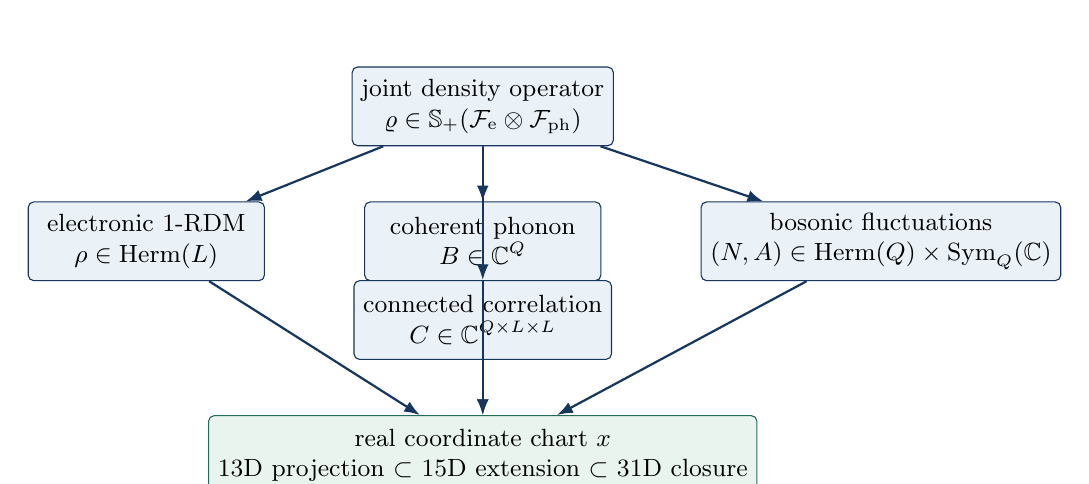
\begin{tikzpicture}[
  node distance=7mm and 11mm,
  every node/.style={font=\small,align=center},
  box/.style={draw=navy,rounded corners=2pt,fill=paleblue,
              minimum width=30mm,minimum height=10mm},
  arr/.style={-{Latex[length=2mm]},thick,navy}
]
\node[box] (full) {joint density operator\\
\(\varrho\in\PSD(\mathcal F_{\rm e}\otimes\mathcal F_{\rm ph})\)};
\node[box,below left=of full] (rho) {electronic 1-RDM\\
\(\rho\in\Herm(L)\)};
\node[box,below=of full] (b) {coherent phonon\\
\(B\in\C^Q\)};
\node[box,below right=of full] (mom) {bosonic fluctuations\\
\((N,A)\in\Herm(Q)\times\Sym_Q(\C)\)};
\node[box,below=17mm of full] (corr) {connected correlation\\
\(C\in\C^{Q\times L\times L}\)};
\node[box,below=of corr,fill=palegreen,draw=green] (coords) {real coordinate
chart \(x\)\\13D projection \(\subset\) 15D extension \(\subset\) 31D closure};

\draw[arr] (full) -- (rho);
\draw[arr] (full) -- (b);
\draw[arr] (full) -- (mom);
\draw[arr] (full) -- (corr);
\draw[arr] (rho) -- (coords);
\draw[arr] (b) -- (coords);
\draw[arr] (mom) -- (coords);
\draw[arr] (corr) -- (coords);
\end{tikzpicture}%
}
\caption{Object-first architecture.  The reduced objects are expectation
values of the full state.  Scalarization is a coordinate chart on a chosen
matrix subspace; it is not an additional physical approximation unless the
chosen subspace fails to be invariant.}
\label{fig:objects}
\end{figure}

\flowlead{Degree counting for the two-site, two-mode closure}

For \(L=Q=2\), the invariant real coordinate set used in the final
diagnostic has
\[
\underbrace{3}_{\rho}
+\underbrace{4}_{B}
+\underbrace{4}_{N}
+\underbrace{6}_{A}
+\underbrace{14}_{C}
=31
\]
real degrees of freedom.  The electronic trace is fixed.  The correlation
sector carries a shared complex trace and two unrestricted complex
\(2\times2\) directions subject to the invariant trace relation implemented
in the dimer closure.

\implementationbox{The local code stores a
\texttt{MatrixDimerState} containing arrays with shapes
\((2,2)\), \((2,)\), \((2,2)\), \((2,2)\), and \((2,2,2)\).  A packing map
converts admissible matrix coordinates to real ODE coordinates.  The
31-coordinate chart is explicit, so every derivative can be compared with
the matrix reference without guessing signs or conjugations.}

\part{What Eqs.~(14a)--(14e) do}

\flowlead{One coupled velocity field, five object sectors}

Reference~\cite{riva2026} derives a second-order equal-time closure for
electron--phonon dynamics.  In our active notation, its architecture is
\[
\begin{array}{rcll}
\dot\rho&=&F_\rho(\rho,B,C),&\text{Eq.~(14a)},\\
\dot N&=&F_N(N,C),&\text{Eq.~(14b)},\\
\dot A&=&F_A(A,C),&\text{Eq.~(14c)},\\
\dot C&=&F_C(C;\rho,N,A,B),&\text{Eq.~(14d)},\\
\dot B&=&F_B(B,\rho),&\text{Eq.~(14e)}.
\end{array}
\]
The semicolon emphasizes that Eq.~(14d) is linear in \(C\) when the other
sectors are prescribed, although the simultaneous system is nonlinear.

\begin{figure}[t]
\centering
\resizebox{0.98\linewidth}{!}{%
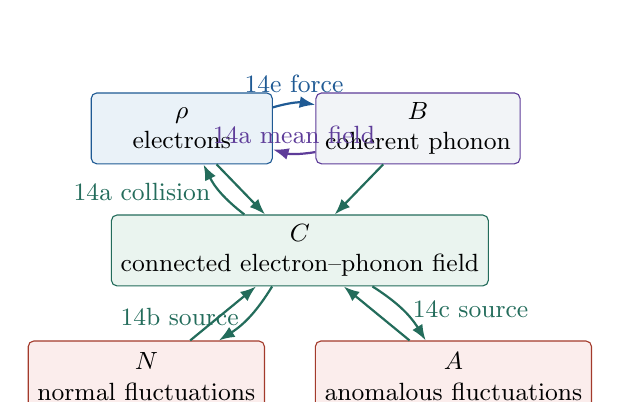
\begin{tikzpicture}[
  every node/.style={font=\small,align=center},
  box/.style={draw,rounded corners=2pt,minimum width=23mm,minimum height=9mm},
  arr/.style={-{Latex[length=2mm]},thick},
  feedback/.style={-{Latex[length=2mm]},thick,bend left=13}
]
\node[box,draw=blue,fill=paleblue] (rho) at (0,0) {\(\rho\)\\electrons};
\node[box,draw=purple,fill=pale] (b) at (3.0,0) {\(B\)\\coherent phonon};
\node[box,draw=green,fill=palegreen] (c) at (1.5,-1.55) {\(C\)\\connected
electron--phonon field};
\node[box,draw=brick,fill=palered] (n) at (-0.45,-3.15) {\(N\)\\normal
fluctuations};
\node[box,draw=brick,fill=palered] (a) at (3.45,-3.15) {\(A\)\\anomalous
fluctuations};

\draw[feedback,blue] (rho) to node[above]{14e force} (b);
\draw[feedback,purple] (b) to node[above]{14a mean field} (rho);
\draw[arr,green] (rho) -- (c);
\draw[arr,green] (b) -- (c);
\draw[arr,green] (n) -- (c);
\draw[arr,green] (a) -- (c);
\draw[feedback,green] (c) to node[left]{14a collision} (rho);
\draw[feedback,green] (c) to node[left]{14b source} (n);
\draw[feedback,green] (c) to node[right]{14c source} (a);
\end{tikzpicture}%
}
\caption{The feedback graph.  The connected field \(C\) is the memory carrier.
It is sourced by the instantaneous electron and phonon moments and then feeds
back into their future velocities.}
\label{fig:feedback}
\end{figure}

The graph should be read as one closed causal circuit.  At a time \(t\),
\((\rho,B,N,A)\) determine the source and transport coefficients in
Eq.~(14d); Eq.~(14d) advances \(C\); and the updated \(C\) changes the
velocities of \(\rho,N,A\) through Eqs.~(14a)--(14c).  Repeating this local
cycle accumulates the past into the present correlation field.  Throughout
the component formulas below, \(1,2,3\) label electronic orbitals and
\(q,q'\) label phonon modes.  Every displayed summation therefore contracts a
declared electronic or phononic index; none of these labels is a power.

\flowlead{Equation (14a): electron transport}

Let
\[
\widetilde h(t)
=h(t)+\sum_q G_q\bigl(B_q+B_q^\ast\bigr)
\]
be the electron Hamiltonian dressed by the coherent phonon.  The dimer
implementation has the source-faithful form
\[
\dot\rho
=-\ii[\widetilde h,\rho]
+\Phi_C+\Phi_C^\dagger,
\tag{14a$'$}
\]
where, in explicit indices,
\[
(\Phi_C)_{12}
=-\ii\sum_{q3}
\left[
(G_q)_{13}C^q_{32}
+(G_q)_{31}(C^q_{23})^\ast
\right].
\]
The commutator transports the electronic density unitarily for prescribed
\(\widetilde h\).  The \(C\)-dependent part transfers population and coherence
through electron--phonon scattering.

The two pieces have different algebraic responsibilities.  Since
\(\Tr[X,Y]=0\), the commutator preserves the electronic trace.  Hermiticity
is preserved because \(-\ii[\widetilde h,\rho]\) is Hermitian when
\(\widetilde h\) and \(\rho\) are Hermitian, and the collision term is written
as \(\Phi_C+\Phi_C^\dagger\).  Thus any later loss of an electronic
eigenvalue occurs inside a trace-preserving Hermitian evolution; it cannot be
diagnosed from trace or Hermiticity checks alone.

\physicalbox{When Eq.~(14d) is formally solved and substituted into
Eq.~(14a), the feedback produces the Fan--Migdal electronic self-energy
described by Ref.~\cite{riva2026}.  The non-Markovian content is therefore not
an optional memory kernel added afterward; it is already encoded in the
coupled equal-time variable \(C\).}

\flowlead{Equation (14b): normal phonon fluctuations}

With mode frequencies \(\omega_q\), the normal covariance obeys
\[
\dot N_{qq'}
=-\ii(\omega_q-\omega_{q'})N_{qq'}
+S^N_{qq'}(C),
\tag{14b$'$}
\]
where the dimer matrix reference resolves the source into
\[
S^N_{qq'}=S^{N,-}_{qq'}+S^{N,+}_{qq'}
\]
with one branch linear in \(C^q\) and the other in
\((C^{q'})^\ast\).  The exact index formula depends on the coupling convention;
the implemented local-Holstein expression is
\[
\begin{aligned}
S^{N,-}_{qq'}
&=-\ii s\sum_{12}
\bigl[-(G_{q'})_{12}\bigr]C^q_{21},\\
S^{N,+}_{qq'}
&=-\ii s\sum_{12}(G_q)_{12}(C^{q'}_{21})^\ast,
\end{aligned}
\tag{2.1}
\]
with spin-degeneracy factor \(s=2\) under the documented dimer convention.
The first branch contracts the \(q\)-correlation with the coupling of mode
\(q'\); the second contracts the conjugated \(q'\)-correlation with the
coupling of mode \(q\).  Their combined index exchange is what preserves
\(N=N^\dagger\).  At equal local frequencies, the free phase
\(-\ii(\omega_q-\omega_{q'})N_{qq'}\) vanishes, so the correlation field
alone controls the instantaneous normal-moment velocity used in the boundary
calculation.

\commentarybox{At the boundary event analyzed later, these two branches make
equal outward contributions.  Equation~(14b) is therefore the
\emph{instantaneous doorway} through which the bosonic cone is crossed.  That
does not yet identify which earlier Eq.~(14d) source created the responsible
correlation field.}

\flowlead{Equation (14c): anomalous fluctuations}

The anomalous covariance obeys
\[
\dot A_{q'q}
=-\ii(\omega_{q'}+\omega_q)A_{q'q}
+S^A_{q'q}(C).
\tag{14c$'$}
\]
For the local dimer reference,
\[
S^A_{q'q}
=-\ii s\sum_{12}
\left[(G_q)_{12}C^{q'}_{12}
      +(G_{q'})_{12}C^q_{12}\right].
\tag{2.2}
\]
The matrix is complex symmetric, \(A=A^{\mathsf T}\).
The two summands exchange \(q\) and \(q'\); this makes the source symmetric
under the same exchange.  Its free phase contains
\(\omega_q+\omega_{q'}\), so anomalous correlations rotate even for
degenerate modes.  The later cone derivative will keep this contribution
separate from the normal source because \(N\) and \(A\) occupy different
blocks of the lifted moment matrix.

\intuition{\(N\) counts centered excitations and mode coherences.
\(A\) records pair-like fluctuations such as
\(\langle\delta b_q\delta b_{q'}\rangle\).  A physical bosonic state restricts
them jointly.  Checking only \(N\succeq0\) misses that coupled uncertainty
condition.}

\flowlead{Equation (14d): the memory carrier}

Along a prescribed \((\rho,N,A,B)\) history, the correlation equation can be
written exactly as
\[
\dot C=\mathcal L(t)C+\sum_{\alpha}S_\alpha(t).
\tag{2.3}
\]
For the dimer transcription, \(\mathcal L C\) contains electronic transport,
the coherent mean field, and the free phonon rotation.  The independent
sources are
\[
\begin{aligned}
S_0^q&=-\ii(\I-\rho)G_q^{\mathsf T}\rho,
&&\text{bare Pauli-blocking source},\\
S_1^q&=-\ii\sum_{q'}N_{qq'}
(\I-\rho)G_{q'}^{\mathsf T}\rho,
&&\text{normal particle source},\\
S_2^q&=+\ii\sum_{q'}N_{qq'}
\rho G_{q'}^{\mathsf T}(\I-\rho),
&&\text{normal hole source},
\end{aligned}
\tag{2.4}
\]
together with two \(A\)-dependent anomalous sources whose explicit index form
is
\[
\begin{aligned}
(S_3^q)_{12}
&=-\ii\sum_{q'3}(G_{q'})_{23}A_{q'q}\rho_{31},\\
(S_4^q)_{12}
&=+\ii\sum_{q'3}(G_{q'})_{32}A_{q'q}\rho_{13}.
\end{aligned}
\tag{2.5}
\]

\physicalbox{The factors \(\rho\) and \(\I-\rho\) implement occupied and
available electronic directions.  Their multiplication by \(N\) or \(A\)
makes Eq.~(14d) nonlinear in the simultaneous state.  The suspected ``strong
nonlinear terms'' are real participants in the dynamics.  The later causal
calculation will show that their paired histories nearly cancel at the first
bosonic boundary crossing of the pinned protocol.}

\flowlead{Equation (14e): coherent phonon motion}

For a prescribed electronic density,
\[
\dot B_q=-\ii\omega_qB_q-\ii s\sum_{12}(G_q)_{12}\rho_{12}.
\tag{14e$'$}
\]
Its exact forced-oscillator form is
\[
\begin{aligned}
B_q(t)
={}&e^{-\ii\omega_q(t-t_0)}B_q(t_0)\\
&-\ii\int_{t_0}^{t}e^{-\ii\omega_q(t-s)}
s\sum_{12}(G_q)_{12}\rho_{12}(s)\,\dd s.
\end{aligned}
\tag{2.6}
\]

\flowlead{Where the memory comes from}

Let \(U(t,s)\) solve
\[
\partial_tU(t,s)=\mathcal L(t)U(t,s),
\qquad U(s,s)=\I.
\tag{2.7}
\]
For one combined source \(S(t)=\sum_\alpha S_\alpha(t)\), multiply
Eq.~(2.3) by the inverse propagator \(U(t_0,t)=U(t,t_0)^{-1}\).  The product
rule, applied to \(Y(t)=U(t_0,t)C(t)\), gives the missing intermediate step:
\[
\begin{aligned}
\dot Y
&=\dot U(t_0,t)C(t)+U(t_0,t)\dot C(t)\\
&=-U(t_0,t)\mathcal L(t)C(t)\\
&\quad+U(t_0,t)\!\left[\mathcal L(t)C(t)+S(t)\right]\\
&=U(t_0,t)S(t).
\end{aligned}
\tag{2.8}
\]
Integrating from \(t_0\) to \(t\) and left-multiplying by \(U(t,t_0)\)
produces
\[
C(t)=U(t,t_0)C(t_0)
+\sum_\alpha\int_{t_0}^{t}U(t,s)S_\alpha(s)\,\dd s,
\tag{2.9}
\]
where
\[
U(t,s)=\mathcal T\exp\!\left[
\int_s^t\mathcal L(\tau)\,\dd\tau
\right].
\tag{2.10}
\]
Substituting Eq.~(2.9) into Eqs.~(14a)--(14c) produces explicit history
integrals.  This is the closed \emph{formal} solution used for causal
attribution.

\commentarybox{The cancellation in Eq.~(2.8) is the algebraic origin of the
history representation.  The propagator removes the homogeneous motion,
leaving only the source created at each intermediate time.  Multiplication by
\(U(t,t_0)\) then returns every created piece to the common endpoint frame.
Because all pieces use the same propagator, their final sum is an exact
decomposition of the realized \(C(t)\) along that trajectory.}

\pedbox{Closed form, carefully stated.}{Equations~(14b), (14c), and (14e)
have exact forced-oscillator integral forms when their sources are prescribed.
Equation~(14d) has a time-ordered variation-of-constants form.  These formulas
close each sector conditionally.  They do not turn the mutually coupled
nonlinear system into a general elementary function of time.}

\implementationbox{A history label \(\alpha\) can be propagated by solving
\(\dot C_\alpha=\mathcal L(t)C_\alpha+S_\alpha(t)\) along the already realized
trajectory.  Linearity in \(C\) guarantees that
\(C=\sum_\alpha C_\alpha\), up to solver error.  The same linear boundary-flux
functional can then be applied to every \(C_\alpha\).}

\part{Scalarization without losing the objects}

\flowlead{Why begin with scalars?}

A scalar-first approach is useful because it makes signs, cancellations,
invariants, and unstable directions inspectable.  Its scientific validity
depends on two separate questions:
\begin{enumerate}
  \item Does the scalar vector field equal the coordinate projection of the
  matrix vector field?
  \item Is the selected scalar coordinate subspace invariant under that
  vector field?
\end{enumerate}
Passing the first test and failing the second means the scalar equations are
correct for the retained components while still omitting generated
directions.

\pedbox{Map-and-arrow chain.}{Matrix state
\(\xrightarrow{\;\Pi\;}\) scalar coordinates
\(\xrightarrow{\;f\;}\) scalar velocity should agree with matrix state
\(\xrightarrow{\;F\;}\) matrix velocity
\(\xrightarrow{\;\Pi\;}\) scalar velocity:
\[
f(\Pi X,t)=\Pi F(X,t).
\]
Invariance adds the requirement that \(F(X,t)\) remain tangent to the embedded
scalar subspace.}

Write \(\mathcal E:\R^d\to\mathcal X\) for the embedding that reconstructs
the matrix state from its real coordinates and
\(\Pi:\mathcal X\to\R^d\) for the packing map, with
\(\Pi\mathcal E=I_d\).  Two residuals make the preceding questions
computable:
\[
\begin{aligned}
r_{\rm par}(x,t)
&=f(x,t)-\Pi F(\mathcal E x,t),\\
r_{\perp}(x,t)
&=\left(I_{\mathcal X}-\mathcal E\Pi\right)
F(\mathcal E x,t).
\end{aligned}
\tag{3.1}
\]
The first residual tests whether the scalar equations reproduce the retained
matrix components.  The second measures the matrix velocity discarded by the
chosen chart.  Hence \(r_{\rm par}=0\) establishes transcription parity, and
\(r_{\perp}=0\) establishes tangency and therefore closure of the embedded
subspace.

The packing operation itself is elementary and exact.  For example,
\[
\begin{aligned}
\begin{pmatrix}a&b+\ii c\\b-\ii c&d\end{pmatrix}
&\in\Herm(2)
\longleftrightarrow (a,d,b,c)\in\R^4,\\
\begin{pmatrix}
\alpha+\ii\beta&\mu+\ii\nu\\
\mu+\ii\nu&\delta+\ii\epsilon
\end{pmatrix}
&\in\Sym_2(\C)
\longleftrightarrow
(\alpha,\beta,\delta,\epsilon,\mu,\nu)\in\R^6.
\end{aligned}
\tag{3.2}
\]
Scalarization becomes an approximation only when the embedding excludes a
direction that the matrix velocity generates, which is precisely what
\(r_\perp\) detects.

\flowlead{The 13-coordinate projection}

The first dimer reduction stores
\[
\begin{aligned}
x_{13}={}&(\Delta n,\rho_{\rm R},\rho_{\rm I},
\Delta B_{\rm R},\Delta B_{\rm I},n_{\rm ph},r_{\rm ph},\\
&d_{\rm R},d_{\rm I},
d_{\rm I}^{+},d_{\rm I}^{-},
d_{\rm R}^{+},d_{\rm R}^{-}).
\end{aligned}
\tag{3.3}
\]
Its electronic embedding is
\[
\rho=
\begin{pmatrix}
(1+\Delta n)/2&\rho_{\rm R}+\ii\rho_{\rm I}\\
\rho_{\rm R}-\ii\rho_{\rm I}&(1-\Delta n)/2
\end{pmatrix}.
\tag{3.4}
\]
The relative coherent mode and symmetric normal covariance are
\[
B=\frac{\Delta B}{2}(1,-1),\qquad
N=
\begin{pmatrix}
n_{\rm ph}&r_{\rm ph}\\
r_{\rm ph}&n_{\rm ph}
\end{pmatrix}.
\tag{3.5}
\]
The six real \(d\)-coordinates encode a traceless correlation matrix
\(C^1\), with \(C^2=-C^1\).

\evidencebox{Across 100 seeded basic-admissible random states, all 13 retained
derivatives matched an independent loop implementation of the matrix
Eqs.~(14a), (14b), (14d), and (14e) to floating-point precision.  This
strongly disfavors a retained-coordinate sign, conjugation, spin-factor, or
normalization transcription error.}

\flowlead{Why the 13D chart is not closed}

The 13-coordinate embedding sets \(A=0\).  Equation~(14c) immediately
generates a nonzero anomalous covariance, so that slice is not invariant.
Dimer symmetry first generates only one complex relative-mode coordinate:
\[
A=\frac{m_-}{2}
\begin{pmatrix}1&-1\\-1&1\end{pmatrix},
\qquad
m_-=m_{\rm R}+\ii m_{\rm I}.
\tag{3.6}
\]
Its reduced equations are
\[
\dot m_{\rm R}=2\omega_{\rm ph}m_{\rm I}+8g\,d_{\rm I},
\qquad
\dot m_{\rm I}=-2\omega_{\rm ph}m_{\rm R}-8g\,d_{\rm R}.
\tag{3.7}
\]
Adding \((m_{\rm R},m_{\rm I})\) gives the 15-coordinate extension.

\evidencebox{The 15 projected derivatives agree with the matrix reference to
floating-point precision.  Under Hartree--Fock initialization, adding these
coordinates delays the late amplitude threshold beyond \(t=360\), yet it does
not prevent early loss of the full bosonic uncertainty condition.}

\flowlead{The 31-coordinate invariant closure}

The final local closure keeps every dimer direction generated by the matrix
equations:
\[
x_{31}
=x_\rho\oplus x_B\oplus x_N\oplus x_A\oplus x_C
\in\R^{3}\oplus\R^{4}\oplus\R^{4}\oplus\R^{6}\oplus\R^{14}.
\tag{3.8}
\]
The normal covariance is an unrestricted Hermitian \(2\times2\) matrix,
\[
N=
\begin{pmatrix}n_1&r+\ii s\\r-\ii s&n_2\end{pmatrix},
\tag{3.9}
\]
and the anomalous covariance is an unrestricted complex symmetric matrix,
\[
A=
\begin{pmatrix}
a_1+\ii b_1&a_{12}+\ii b_{12}\\
a_{12}+\ii b_{12}&a_2+\ii b_2
\end{pmatrix}.
\tag{3.10}
\]
The correlation chart retains a shared complex trace and six additional real
coordinates for each mode.  Projection after every matrix derivative
reproduces all 31 scalar derivatives.

\begin{table*}[t]
\centering
\caption{The nested scalar models and the scientific question answered by
each.}
\label{tab:closures}
\begin{tabularx}{0.94\textwidth}{@{}p{0.10\textwidth}p{0.20\textwidth}Y Y@{}}
\toprule
Chart & Retained objects & What it establishes & What it omits \\
\midrule
13D & Symmetry-reduced \(\rho,B,N,C\), with \(A=0\) &
Direct readability and parity of the retained equations &
Eq.~(14c) points out of the embedded slice.\\
15D & 13D plus one complex relative anomalous mode &
Minimal Eq.~(14c) parity and its delayed amplitude threshold &
Other normal, anomalous, coherent, and correlation directions.\\
31D & Full generated two-site matrix directions in real coordinates &
Invariant matrix--scalar closure for the tested symmetry and trace sector &
Higher moments absent from the second-order physical closure itself.\\
\bottomrule
\end{tabularx}
\end{table*}

\commentarybox{Scalarization is therefore the correct diagnostic instrument
only after the coordinate chart is made invariant.  The 31D chart preserves
matrix meaning while giving every source a real coordinate address.}

The nesting \(13\subset15\subset31\) is consequently a cumulative sequence of
diagnostic questions.  The 13D chart exposes
the first signs and cancellations; the 15D chart proves that Eq.~(14c)
immediately generates an omitted anomalous direction; the 31D chart removes
every discarded direction found by the dimer matrix audit.  Once the last
embedding satisfies both residual tests in Eq.~(3.1), a scalar instability is
the instability of the tested matrix closure written in real coordinates.

\begin{table*}[t]
\centering
\caption{Matched 15D event times after the complex anomalous relative mode is
added.  A dash denotes survival through \(t=400\).}
\label{tab:15devents}
\begin{tabularx}{0.86\textwidth}{@{}Yrrr@{}}
\toprule
Protocol & Boson uncertainty event & Electron PSD event & Amplitude event\\
\midrule
HF, zero \(C\) & \(1.37720\) & \(41.5049\) & \(366.6906\)\\
Exact contractions & \(6.13867\) & \(1.01873\) & \(132.7035\)\\
Exact plus Eq.~(3.12) & \(3.68211\) & --- & ---\\
\bottomrule
\end{tabularx}
\end{table*}

\begin{figure*}[t]
\centering
\begin{minipage}[t]{0.485\textwidth}
\centering
\includegraphics[width=\linewidth]{eq14c_protocols.pdf}\\[-2pt]
\small\textbf{(a)} Amplitude evolution.
\end{minipage}\hfill
\begin{minipage}[t]{0.485\textwidth}
\centering
\includegraphics[width=\linewidth]{eq14c_uncertainty.pdf}\\[-2pt]
\small\textbf{(b)} Relative-mode uncertainty margin.
\end{minipage}
\caption{The 15D extension delays the HF amplitude threshold from
\(t\approx130.47\) to \(t\approx366.69\), yet every tested protocol reaches a
bosonic uncertainty boundary first.  The zero line in panel (b) is the
condition \(n_-(n_-+1)-|m_-|^2=0\).}
\label{fig:15dprotocols}
\end{figure*}

\flowlead{Initialization and the residual-subtraction experiment}

Let the autonomous or driven scalar system be
\[
\dot x=F(x,t).
\tag{3.11}
\]
The local dimer notes introduce the diagnostic modification
\[
\dot x=F(x,t)-F(x_0,0).
\tag{3.12}
\]
This is called Eq.~(112) in those notes.  It forces
\(\dot x(0)=0\) before the pulse because the initial residual is subtracted as
a constant vector.

\intuition{The operation pins the chosen initial coordinate to the modified
undriven vector field.  It changes every later velocity by the same
sector-wise vector.  It is therefore a dynamical intervention, not merely a
better numerical solver or a re-labeling of the initial state.}

For exact ground-state contractions in the truncated second-order closure,
the full-EOM residual is not zero.  At phonon cutoff 16 and the pinned strong
parameters, the exact dimer energy and its reconstruction from the retained
objects agree to about \(10^{-14}\), while the approximate full-EOM RHS norm
is about \(0.3714\).  Exactness of the many-body state does not make its
truncated moments a fixed point of an approximate moment closure.

\begin{table}[h]
\centering
\caption{Initialization outcomes in the earlier scalar diagnostic.  Times are
in \(t_{\rm hop}^{-1}\).}
\begin{tabularx}{\linewidth}{@{}Yrr@{}}
\toprule
Protocol & Amplitude event & Electron PSD event\\
\midrule
HF, zero \(C\) & \(130.47\) & \(15.5177\)\\
Stationary root & none through 400 & \(30.5557\)\\
Exact contractions & \(154.25\) & \(0.9909\)\\
Exact plus Eq.~(3.12) & none through 400 & none through 400\\
\bottomrule
\end{tabularx}
\end{table}

\warningbox{The last row was encouraging in the reduced scalar checks, but
those checks did not yet test the coupled \(N,A\) uncertainty cone.  The 31D
closure reveals an earlier bosonic failure.}

\begin{figure*}[t]
\centering
\begin{minipage}[t]{0.485\textwidth}
\centering
\includegraphics[width=\linewidth]{initialization_protocols.pdf}\\[-2pt]
\small\textbf{(a)} Matched 13D amplitude histories.
\end{minipage}\hfill
\begin{minipage}[t]{0.485\textwidth}
\centering
\includegraphics[width=\linewidth]{regularized_physicality.pdf}\\[-2pt]
\small\textbf{(b)} Reduced 13D positivity checks after Eq.~(3.12).
\end{minipage}
\caption{Correlated initialization and residual subtraction suppress the late
13D amplitude event.  Panel (b) monitors the electronic 1-RDM and the retained
normal-phonon density; the anomalous field \(A\) is absent from this chart, so
these positive curves cannot certify the full bosonic moment cone.}
\label{fig:13dprotocols}
\end{figure*}

\part{The bosonic physical cone}

\flowlead{From moments to one positive matrix}

Collect the centered phonon operators into
\[
\xi=
\begin{pmatrix}
\delta b^\dagger\\
\delta b
\end{pmatrix}.
\tag{4.1}
\]
The block entries follow from operator ordering, including the identity term
that is easy to lose in a purely matrix-level transcription:
\[
\begin{aligned}
\left\langle\delta b_q^\dagger\delta b_{q'}\right\rangle
&=N_{q'q}=(N^{\mathsf T})_{qq'},\\
\left\langle\delta b_q^\dagger\delta b_{q'}^\dagger\right\rangle
&=A_{qq'}^\ast,\\
\left\langle\delta b_q\delta b_{q'}\right\rangle
&=A_{qq'},\\
\left\langle\delta b_q\delta b_{q'}^\dagger\right\rangle
&=\delta_{qq'}
  \left\langle\delta b_{q'}^\dagger\delta b_q\right\rangle
=(\I+N)_{qq'}.
\end{aligned}
\tag{4.2}
\]
Their second-moment matrix is
\[
\MB
=\langle\xi\xi^\dagger\rangle
=
\begin{pmatrix}
N^{\mathsf T}&A^\ast\\
A&\I+N
\end{pmatrix}.
\tag{4.3}
\]
For any \(z\in\C^{2Q}\),
\[
z^\dagger\MB z
=\left\langle
(z^\dagger\xi)(z^\dagger\xi)^\dagger
\right\rangle
\geq0.
\tag{4.4}
\]
Therefore every physical state satisfies
\[
\boxed{\MB\succeq0.}
\tag{4.5}
\]

\intuition{Choose any complex linear combination of centered creation and
annihilation operators.  Equation~(4.4) is the expectation value of an
operator multiplied by its adjoint, so it cannot be negative.  A negative
eigenvalue of \(\MB\) would claim that some squared fluctuation has negative
expectation value.}

\flowlead{One-mode example}

For one mode, write \(N=n\) and \(A=m\).  Then
\[
\MB=
\begin{pmatrix}
n&m^\ast\\m&n+1
\end{pmatrix}.
\tag{4.6}
\]
Positive semidefiniteness requires
\[
n\geq0,\qquad n(n+1)-|m|^2\geq0.
\tag{4.7}
\]
Thus a nonnegative occupation \(n\) is insufficient.  The anomalous magnitude
must also obey
\[
|m|^2\leq n(n+1).
\tag{4.8}
\]

\physicalbox{Equation~(4.8) is the simplest picture of the coupled
uncertainty constraint.  A large pair correlation \(m\) needs enough normal
fluctuation \(n\) to support it.  The 13D model could pass \(N\succeq0\) while
missing a failure of this joint condition because it had set \(A=0\).}

\flowlead{Geometry of the boundary}

The physical bosonic moment set is the preimage
\[
\mathcal K_{\rm B}
=\{(N,A):\MB(N,A)\succeq0\}.
\tag{4.9}
\]
It is convex because the lift \((N,A)\mapsto\MB\) is affine and the PSD cone
is convex.  The derivative lift is the linear map
\[
\LB(\dot N,\dot A)
=\dot\MB
=
\begin{pmatrix}
\dot N^{\mathsf T}&\dot A^\ast\\
\dot A&\dot N
\end{pmatrix}.
\tag{4.10}
\]

\begin{figure}[t]
\centering
\resizebox{0.98\linewidth}{!}{%
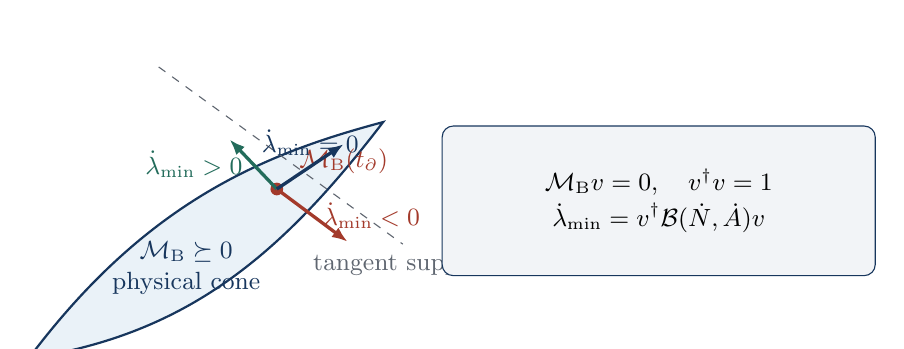
\begin{tikzpicture}[
  every node/.style={font=\small,align=center},
  arr/.style={-{Latex[length=2mm]},very thick}
]
\draw[thick,navy,fill=paleblue]
  (0,0) .. controls (2.0,0.3) and (3.2,1.3) .. (4.5,3.0)
  .. controls (3.0,2.6) and (1.5,2.0) .. (0,0);
\node[navy] at (2.0,1.15) {\(\MB\succeq0\)\\physical cone};
\fill[brick] (3.15,2.15) circle (2.3pt);
\node[brick] at (4.0,2.50) {\(\MB(t_\partial)\)};
\draw[dashed,muted] (1.65,3.7) -- (4.75,1.45);
\node[muted] at (4.75,1.18) {tangent support};
\draw[arr,green] (3.15,2.15) -- (2.55,2.78)
  node[midway,left] {\(\dot\lambda_{\min}>0\)};
\draw[arr,brick] (3.15,2.15) -- (4.05,1.48)
  node[midway,right] {\(\dot\lambda_{\min}<0\)};
\draw[arr,navy] (3.15,2.15) -- (4.0,2.72)
  node[midway,above] {\(\dot\lambda_{\min}=0\)};

\node[draw=navy,rounded corners,fill=pale,minimum width=55mm,
      minimum height=19mm] at (8.0,2.0)
{\(\MB v=0,\quad v^\dagger v=1\)\\[2pt]
\(\displaystyle\dot\lambda_{\min}
=v^\dagger\LB(\dot N,\dot A)v\)};
\end{tikzpicture}%
}
\caption{Cone geometry at a simple boundary eigenvalue.  The sign of the
null-mode flux determines whether the vector field points inward, tangent, or
outward to first order.}
\label{fig:cone}
\end{figure}

\flowlead{Deriving the boundary flux}

Suppose the smallest eigenvalue is simple near \(t_\partial\):
\[
\MB(t)v(t)=\lambda(t)v(t),\qquad v^\dagger v=1.
\tag{4.11}
\]
Differentiate:
\[
\dot\MB v+\MB\dot v=\dot\lambda\,v+\lambda\dot v.
\tag{4.12}
\]
Left-multiply by \(v^\dagger\).  Hermiticity gives
\(v^\dagger\MB=\lambda v^\dagger\), so the terms containing \(\dot v\)
cancel:
\[
\boxed{\dot\lambda=v^\dagger\dot\MB v.}
\tag{4.13}
\]
Writing the normalized eigenvector in creation/annihilation blocks,
\(v=(u,w)^{\mathsf T}\) with \(u,w\in\C^Q\), now exposes the contribution of
each moment equation:
\[
\begin{aligned}
\dot\lambda
&=
\begin{pmatrix}u^\dagger&w^\dagger\end{pmatrix}
\begin{pmatrix}
\dot N^{\mathsf T}&\dot A^\ast\\
\dot A&\dot N
\end{pmatrix}
\begin{pmatrix}u\\w\end{pmatrix}\\
&=u^\dagger\dot N^{\mathsf T}u
  w^\dagger\dot Nw
  2\Re\!\left(w^\dagger\dot A\,u\right).
\end{aligned}
\tag{4.14}
\]
The first two terms are the lifted Eq.~(14b) velocity, and the last term is
the lifted Eq.~(14c) velocity.  Equation~(14d) enters this first derivative
only through the already accumulated value of \(C\) appearing in
\(\dot N\) and \(\dot A\).

At the boundary, \(\lambda=0\).  The signs mean
\[
\begin{array}{ccl}
\dot\lambda>0&:&\text{inward to first order},\\
\dot\lambda=0&:&\text{tangent to first order},\\
\dot\lambda<0&:&\text{outward to first order}.
\end{array}
\tag{4.15}
\]

\commentarybox{Equation~(4.13) converts a matrix representability question
into one scalar.  The vector \(v\) selects the fluctuation combination that
has just run out of physical variance; the quadratic form measures the
instantaneous velocity of that variance.}

\flowlead{Degenerate boundary modes}

If the zero eigenvalue has multiplicity \(r>1\), one vector is insufficient.
Let \(P_0\) project onto \(\ker\MB\).  The first-order tangent condition is
\[
P_0\dot\MB P_0\succeq0.
\tag{4.16}
\]
The reproduced crossing has a simple lowest eigenvalue: the next eigenvalue
is approximately \(0.19436\).  Equation~(4.13) is therefore the appropriate
first-order diagnostic for that event.

\implementationbox{Compute the Hermitian \(\MB\) with
\texttt{eigh}, locate the first sign change of its smallest eigenvalue with a
dense solver output or event refinement, normalize the associated eigenvector,
evaluate every stored RHS contribution, lift each \((\dot N,\dot A)\) by
Eq.~(4.10), and form \(v^\dagger(\cdot)v\).  The contributions must reconstruct
the total to the same numerical tolerance as the RHS split.}

\part{Reproducing and isolating the failure}

\flowlead{Pinned protocol and hierarchy of events}

The main diagnostic trajectory uses:
\begin{itemize}
  \item two electronic sites and two local phonon modes;
  \item \(\lambda=1.5\), \(\gamma=0.5\), and \(v/t_{\rm hop}=1\);
  \item exact ground-state contractions at local phonon cutoff 16;
  \item the 31-real-coordinate invariant closure;
  \item the constant residual subtraction of Eq.~(3.12);
  \item adaptive event refinement for
  \(\lambda_{\min}(\MB)=0\).
\end{itemize}

\begin{table*}[t]
\centering
\caption{Event hierarchy in the invariant 31D closure.  Event times are in
\(t_{\rm hop}^{-1}\); a dash denotes survival through \(t=400\).}
\label{tab:31devents}
\begin{tabularx}{0.88\textwidth}{@{}Yrrr@{}}
\toprule
Protocol & Full boson-cone event & Electron PSD event & Amplitude event\\
\midrule
HF, zero \(C\) & \(1.322700\) & \(27.963400\) & \(54.461296\)\\
Exact contractions & \(3.682070\) & \(1.036206\) & \(141.405587\)\\
Exact plus Eq.~(3.12) & \(1.486956\) & --- & ---\\
\bottomrule
\end{tabularx}
\end{table*}

\begin{figure*}[t]
\centering
\begin{minipage}[t]{0.485\textwidth}
\centering
\includegraphics[width=\linewidth]{closed_scalar_protocols.pdf}\\[-2pt]
\small\textbf{(a)} 31D amplitude histories.
\end{minipage}\hfill
\begin{minipage}[t]{0.485\textwidth}
\centering
\includegraphics[width=\linewidth]{closed_scalar_physicality.pdf}\\[-2pt]
\small\textbf{(b)} Early cone margins for exact contractions plus
Eq.~(3.12).
\end{minipage}
\caption{Amplitude boundedness and representability separate in the invariant
closure.  Eq.~(3.12) keeps \(\max_i|x_i|\leq2.2613\) through \(t=400\), while
the full bosonic moment eigenvalue in panel (b) crosses zero at
\(t_\partial=1.48695622\).}
\label{fig:31dprotocols}
\end{figure*}

The first bosonic boundary occurs at
\[
\boxed{
t_\partial=1.48695622167\,t_{\rm hop}^{-1}.
}
\tag{5.1}
\]
At the crossing,
\[
\boxed{
\dot\lambda_{\min}
=-3.92402267\times10^{-3}.
}
\tag{5.2}
\]
The negative sign establishes an outward crossing for the implemented
second-moment trajectory.

\evidencebox{A centered finite difference of the smallest eigenvalue agrees
with the quadratic-form derivative within \(5\times10^{-10}\) under the
tested tolerances.  Direct summation of the term lifts reconstructs the full
\(\dot\MB\) at the reported precision.}

\flowlead{Instantaneous flux decomposition}

At \(t_\partial\), the signed contributions are
\[
\dot\lambda_{\min}
=\sum_k v^\dagger\dot\MB^{(k)}v.
\tag{5.3}
\]

\begin{center}
\small
\textbf{Instantaneous null-mode flux at the first bosonic boundary.}\par
\smallskip
\begin{tabularx}{\linewidth}{@{}Y r@{}}
\toprule
Contribution & \(v^\dagger\dot\MB^{(k)}v\)\\
\midrule
Eq.~(14b), \(C\) source & \(-3.92638757\times10^{-3}\)\\
Eq.~(14c), \(C\) source & \(+2.23204135\times10^{-6}\)\\
Eq.~(14d), direct & \(0\)\\
Eq.~(112), direct lift & \(+1.32861458\times10^{-7}\)\\
\midrule
Total & \(-3.92402267\times10^{-3}\)\\
\bottomrule
\end{tabularx}
\end{center}

\begin{figure*}[t]
\centering
\includegraphics[width=0.72\textwidth]{boson_boundary_flux.pdf}
\caption{Signed equation-group contributions to
\(v^\dagger\dot{\MB}v\) at the first 31D bosonic boundary.  Eq.~(14b)'s
correlation source supplies the outward rate; Eq.~(14c) and the direct
Eq.~(112) lift are smaller inward contributions, and Eq.~(14d) enters through
the prior evolution of \(C\).}
\label{fig:boundaryflux}
\end{figure*}

Each of the two correlation branches of Eq.~(14b) contributes
\[
-1.96319379\times10^{-3}.
\tag{5.4}
\]
The free Eq.~(14b) rotation vanishes for the degenerate local mode
frequencies, and the free Eq.~(14c) rotation has zero null-mode projection to
numerical precision.

\pedbox{Direct cause versus causal origin.}{Equation~(14b) is the direct
outward velocity because \(\MB\) depends only on \(N\) and \(A\).
Equation~(14d) has no direct entry in \(\dot\MB\), but it creates \(C\), which
then appears in Eqs.~(14b) and (14c).  To attribute Eq.~(14d), we must carry
its sources through their histories.}

\flowlead{Variation-of-constants attribution}

Along the already realized trajectory, split Eq.~(14d) into
\[
\dot C=\mathcal L(t)C
+S_{112}+S_0+S_1+S_2+S_3+S_4.
\tag{5.5}
\]
Define
\[
\begin{aligned}
C_{\rm i}(t)&=U(t,t_0)C(t_0),\\
C_\alpha(t)&=\int_{t_0}^{t}U(t,s)S_\alpha(s)\,\dd s.
\end{aligned}
\tag{5.6}
\]
Then
\[
C(t)=C_{\rm i}(t)+\sum_\alpha C_\alpha(t).
\tag{5.7}
\]
Let \(F_N^C\) and \(F_A^C\) denote the parts of Eqs.~(14b)--(14c) linear in
\(C\).  With the boundary eigenvector held at its realized value, define
\[
\ell_\partial(C)
=v^\dagger
\LB\!\left(F_N^C(C),F_A^C(C)\right)v.
\tag{5.8}
\]
Both \(F_N^C,F_A^C\) and \(\LB\) are linear, so
\(\ell_\partial(C_1+C_2)=\ell_\partial(C_1)+\ell_\partial(C_2)\).
Applying this identity to Eq.~(5.7) gives the final source attribution
\[
\ell_\partial(C(t_\partial))
=\ell_\partial(C_{\rm i})
+\sum_\alpha\ell_\partial(C_\alpha).
\tag{5.9}
\]

\implementationbox{This is an exact decomposition along the selected
numerical trajectory, not a counterfactual rerun.  Every source history sees
the same \(\mathcal L(t)\), \(\rho(t)\), \(N(t)\), \(A(t)\), and \(B(t)\).
Their sum reconstructed the realized boundary correlation with error
\(5.2\times10^{-16}\), and reconstructed its Eq.~(14b) flux with error
\(1.4\times10^{-16}\).}

\flowlead{Source histories at the boundary}

\begin{center}
\small
\textbf{History-resolved Eq.~(14b) boundary flux.}\par
\smallskip
\begin{tabularx}{\linewidth}{@{}Y r@{}}
\toprule
Correlation history & \(\ell_\partial(C_\alpha)\)\\
\midrule
Eq.~(112), correlation-sector subtraction
& \(-1.96942674\times10^{-1}\)\\
Eq.~(14d), bare Pauli-blocking source
& \(+1.93016288\times10^{-1}\)\\
Eq.~(14d), first anomalous source
& \(-4.60900119\times10^{-4}\)\\
Eq.~(14d), second anomalous source
& \(+4.60893147\times10^{-4}\)\\
Eq.~(14d), normal particle source
& \(+2.30146227\times10^{-5}\)\\
Eq.~(14d), normal hole source
& \(-2.30243186\times10^{-5}\)\\
Propagated initial \(C\)
& \(+1.45595687\times10^{-8}\)\\
\midrule
Reconstructed Eq.~(14b) flux
& \(-3.92638757\times10^{-3}\)\\
\bottomrule
\end{tabularx}
\end{center}

The absolute source-history magnitudes sum to approximately
\[
\Sigma_{\rm abs}=0.39093,
\tag{5.10}
\]
while the signed result is about \(0.0039264\) in magnitude.  The cancellation
fraction is
\[
1-\frac{|\sum_\alpha\ell_\partial(C_\alpha)|}
{\sum_\alpha|\ell_\partial(C_\alpha)|}
=0.989956.
\tag{5.11}
\]
Thus
\[
\boxed{\text{the boundary-driving history is \(98.9956\%\) cancellation.}}
\]

The arithmetic is worth reading as a conditioning statement.  If
\(f_\alpha=\ell_\partial(C_\alpha)\), then
\[
\left|\sum_\alpha f_\alpha\right|
\approx3.9264\times10^{-3},
\qquad
\sum_\alpha|f_\alpha|\approx3.9093\times10^{-1}.
\tag{5.12}
\]
Only about one percent of the separately transported magnitude survives in
the signed endpoint flux.  Consequently, an error or initialization-induced
change of size \(10^{-3}\) in one dominant history is small relative to that
history and already comparable with the complete outward residual.

\begin{figure*}[t]
\centering
\includegraphics[width=0.78\textwidth]{eq14d_history_flux.pdf}
\caption{Variation-of-constants attribution at \(t_\partial\).  The upper
panel resolves the dominant cancellation between the Eq.~(112) correlation
subtraction and Eq.~(14d)'s bare Pauli source.  The lower panel enlarges the
paired anomalous and normal histories by \(10^4\); each pair is active and
nearly self-cancelling.}
\label{fig:historybars}
\end{figure*}

\flowlead{The suspected nonlinear pair}

The two anomalous histories sum to
\[
-4.60900119\times10^{-4}
+4.60893147\times10^{-4}
=-6.97\times10^{-9}.
\tag{5.13}
\]
The normal particle and hole histories sum to
\[
+2.30146227\times10^{-5}
-2.30243186\times10^{-5}
=-9.70\times10^{-9}.
\tag{5.14}
\]
These terms are strong enough to be visible separately, but they are not the
dominant \emph{net} driver at this first crossing.

\evidencebox{The Eq.~(112) correlation history and the bare Pauli-blocking
history alone reproduce \(99.99995\%\) of the final signed Eq.~(14b) flux.
The correlation-sector subtraction is outward and about \(2.034\%\) larger in
magnitude than its bare-Pauli opponent.}

\flowlead{Why a tiny imbalance matters}

If two histories are \(a<0\) and \(b>0\), their residual is
\[
r=a+b.
\tag{5.15}
\]
The relative sensitivity to a perturbation \(\delta a\) is
\[
\frac{|\delta r|}{|r|}
=\frac{|\delta a|}{|a+b|}.
\tag{5.16}
\]
Here \(|a|\) and \(|b|\) are about \(0.2\), while \(|r|\) is about \(0.004\).
A percent-scale change in either dominant contribution can therefore change
the sign or timing of the boundary flux by order one relative to the residual.

\intuition{Sensitive initial conditions do not require chaos.  They can arise
when the observable of interest is the small difference between two large,
opposing histories.  Initialization changes the sources, and the memory
propagator transports those changes to the later cancellation.}

\flowlead{The one-sector ablation}

The causal interpretation has a direct counterfactual test:
\begin{center}
\begin{tabularx}{\linewidth}{@{}Y r@{}}
\toprule
Residual-subtraction placement & \(t_\partial\)\\
\midrule
All sectors & \(1.48695622\)\\
Only the \(C\) sector & \(1.48689983\)\\
Every sector except \(C\) & \(3.68307711\)\\
No subtraction, exact contractions & \(\approx3.68207\)\\
\bottomrule
\end{tabularx}
\end{center}
Removing only the constant correlation-sector subtraction nearly restores
the unregularized boundary time.  This isolates the early cone shift to that
sector of Eq.~(3.12).

\warningbox{This ablation does not prove that the full Eq.~(112) intervention
is globally harmful.  In the tested scalar trajectory it suppresses the late
amplitude divergence and preserves electronic positivity.  It also advances
this bosonic representability loss when applied as a constant subtraction in
the correlation equation.  Both statements are true because they measure
different properties.}

\begin{center}
\small
\textbf{Earlier 13D source-pair ablation.}\par
\smallskip
\begin{tabularx}{\linewidth}{@{}Yrr@{}}
\toprule
13D source choice & \(\|F(x_0,0)\|_2\) & Amplitude event\\
\midrule
Both retained & \(0.34233\) & \(130.47\)\\
Eq.~(95) off & \(0.30619\) & \(60.43\)\\
Eq.~(97) off & \(0.15309\) & \(69.67\)\\
Both off & \(0\) & \(59.92\)\\
\bottomrule
\end{tabularx}
\end{center}

\begin{figure}[t]
\centering
\includegraphics[width=\linewidth]{ablation_failure_times.pdf}
\caption{Removing either initially active 13D source accelerates the amplitude
event.  Removing both makes the initial residual vanish and still produces an
event at \(t=59.92\), so the residual norm alone cannot explain the late
growth.}
\label{fig:sourceablation}
\end{figure}

\flowlead{Three phenomena that must remain separate}

\begin{enumerate}
  \item \textbf{Physical cone escape:} a covariance or density matrix obtains
  a negative eigenvalue.  This is the earliest event diagnosed here.
  \item \textbf{Amplitude divergence:} a selected coordinate exceeds a large
  declared threshold, such as \(10^4\).  This is a later numerical symptom in
  some protocols.
  \item \textbf{Chaos:} nearby physical trajectories have a positive
  asymptotic Lyapunov exponent on a bounded invariant set, with supporting
  convergence and structural diagnostics.
\end{enumerate}

\pedbox{Current conclusion.}{The pinned failure is an outward escape from a
bosonic second-moment cone caused by a correlation history with near-perfect
cancellation.  A late nonlinear amplification is also reproducible.  Neither
result establishes a strange attractor.}

\flowlead{Why the ODE solver is not the leading explanation}

\begin{center}
\begin{tabularx}{\linewidth}{@{}Yrr@{}}
\toprule
Integrator & Step or tolerance & Amplitude event\\
\midrule
RK4 & \(\Delta t=0.020\) & \(130.480000\)\\
RK4 & \(\Delta t=0.010\) & \(130.470000\)\\
RK4 & \(\Delta t=0.005\) & \(130.470000\)\\
DOP853 & \(10^{-10}/10^{-12}\) & \(130.467461976\)\\
Radau & \(10^{-10}/10^{-12}\) & \(130.467462019\)\\
BDF & \(10^{-10}/10^{-12}\) & \(130.467318885\)\\
\bottomrule
\end{tabularx}
\end{center}

The RK4 refinement and three adaptive solvers converge to the same late
amplitude event.  The matrix--scalar RHS parity tests reached floating-point
agreement, and the boundary derivative was independently checked by a
centered finite difference.  These tests strongly disfavor coarse time
stepping or a retained-coordinate transcription mistake as the complete
explanation.

\begin{figure*}[t]
\centering
\begin{minipage}[t]{0.485\textwidth}
\centering
\includegraphics[width=\linewidth]{trajectory_max_abs.pdf}\\[-2pt]
\small\textbf{(a)} Strong and weak 13D amplitude histories.
\end{minipage}\hfill
\begin{minipage}[t]{0.485\textwidth}
\centering
\includegraphics[width=\linewidth]{jacobian_growth.pdf}\\[-2pt]
\small\textbf{(b)} Maximum instantaneous Jacobian growth rate.
\end{minipage}
\caption{The strong scalar trajectory enters rapid local amplification near
its amplitude event, while the matched weak-coupling control remains bounded.
Panel (b) contains instantaneous Jacobian eigenvalues along one trajectory;
they are local amplification diagnostics rather than Lyapunov exponents.}
\label{fig:scalarinstability}
\end{figure*}

\commentarybox{A converged solver can faithfully integrate an unphysical
closure trajectory.  Numerical stability and physical representability are
two different contracts.  The next design must enforce the latter without
silently sacrificing conservation or source fidelity.}

\part{Cone-aware correction design}

\flowlead{The design contract}

A useful regularization should do more than keep coordinates finite.  For the
present closure, its minimum contract is:
\begin{enumerate}
  \item preserve \(\rho=\rho^\dagger\), \(0\preceq\rho\preceq\I\), and the
  fixed electronic trace;
  \item preserve \(N=N^\dagger\), \(A=A^{\mathsf T}\), and \(\MB\succeq0\);
  \item retain the source equations in the cone interior;
  \item introduce the smallest possible velocity change near an outward
  boundary;
  \item keep particle number and post-pulse energy drift within declared
  tolerances;
  \item improve or at least retain agreement with exact dimer observables;
  \item remain stable under step, tolerance, cutoff, and parameter refinement.
\end{enumerate}

\evidencebox{A minimal state-dependent correction has been implemented in the
ten real \((\dot N,\dot A)\) coordinates.  The complete matrix barrier is
required when low bosonic modes become nearly degenerate.  A
correlation-sector correction remains the next causal comparison.}

\flowlead{First construction: tangent projection}

Let the unmodified bosonic moment velocity be
\[
D=\LB(\dot N,\dot A)\in\Herm(2Q).
\tag{6.1}
\]
At a simple boundary mode \(v\), choose a desired nonnegative inward margin
\(\kappa\geq0\) and solve
\[
\begin{aligned}
\underset{\Delta D\in\Herm(2Q)}{\text{minimize}}\quad&
\frac12\lVert\Delta D\rVert_{\Frob}^2,\\
\text{subject to}\quad&
v^\dagger(D+\Delta D)v\geq\kappa.
\end{aligned}
\tag{6.2}
\]
The gradient of the constraint functional under the Frobenius inner product
is \(vv^\dagger\), whose squared norm is one.  The solution is
\[
\boxed{
\Delta D
=\bigl[\kappa-v^\dagger Dv\bigr]_+\,vv^\dagger,
}
\tag{6.3}
\]
where \([a]_+=\max(a,0)\).

To derive the projection, first observe that the zero correction is optimal
whenever the uncorrected velocity already satisfies the inequality.  In the
active case, the constraint boundary is
\[
\langle vv^\dagger,\Delta D\rangle_{\Frob}
=\kappa-v^\dagger Dv.
\tag{6.4}
\]
The Lagrangian
\[
\mathcal L_{\rm KKT}(\Delta D,\mu)
=\tfrac12\lVert\Delta D\rVert_{\Frob}^2
-\mu\!\left[
\langle vv^\dagger,\Delta D\rangle_{\Frob}
-\kappa+v^\dagger Dv\right]
\tag{6.4a}
\]
has stationarity condition
\(\Delta D-\mu vv^\dagger=0\).  Since
\(\lVert vv^\dagger\rVert_{\Frob}^2
=\Tr(vv^\dagger vv^\dagger)=1\), substitution into Eq.~(6.4) gives
\(\mu=\kappa-v^\dagger Dv\).  Complementary slackness replaces this active
value by its positive part, thereby proving Eq.~(6.3) without an omitted
optimization step.

\intuition{The correction adds velocity only to the fluctuation direction
that is about to become negative.  It does not push every covariance
coordinate or erase the physical source terms in the cone interior.}

\flowlead{Respecting the structured moment lift}

An arbitrary Hermitian \(\Delta D\) need not have the block structure in
Eq.~(4.10).  Let \(y\in\R^{10}\) collect admissible corrections to a Hermitian
\(\dot N\) and a complex symmetric \(\dot A\) for \(Q=2\).  Define the linear
lift
\[
\mathcal S:y\longmapsto
\begin{pmatrix}
\Delta\dot N^{\mathsf T}&\Delta\dot A^\ast\\
\Delta\dot A&\Delta\dot N
\end{pmatrix}.
\tag{6.5}
\]
The structured quadratic program is
\[
\begin{aligned}
\underset{y\in\R^{10}}{\text{minimize}}\quad&
\frac12 y^{\mathsf T}Wy,\\
\text{subject to}\quad&
v^\dagger\!\left[D+\mathcal S(y)\right]v\geq\kappa,\\
&Ay=0.
\end{aligned}
\tag{6.6}
\]
Here \(W\succ0\) chooses the metric, and \(Ay=0\) encodes linear equalities
such as symmetry-preserving relations or a desired instantaneous energy
condition.

For one active inequality and no equalities, define the real covector
\[
a^{\mathsf T}y=v^\dagger\mathcal S(y)v.
\tag{6.7}
\]
Then the weighted minimum-norm solution is
\[
\boxed{
y_\ast
=\frac{\bigl[\kappa-v^\dagger Dv\bigr]_+}
{a^{\mathsf T}W^{-1}a}\,W^{-1}a.
}
\tag{6.8}
\]

Indeed, with deficit
\(d=[\kappa-v^\dagger Dv]_+\), the active Lagrangian is
\[
\mathcal L_{\rm KKT}(y,\mu)
=\tfrac12y^{\mathsf T}Wy-\mu(a^{\mathsf T}y-d).
\tag{6.8a}
\]
Stationarity and feasibility give the complete KKT chain
\[
\begin{aligned}
Wy-\mu a&=0,
&y&=\mu W^{-1}a,\\
a^{\mathsf T}y&=d,
&\mu&=\frac{d}{a^{\mathsf T}W^{-1}a},
\end{aligned}
\tag{6.8b}
\]
which yields Eq.~(6.8).  If the equality constraints \(Ay=0\) are present,
let the columns of \(Z\) span \(\ker A\) and write \(y=Zq\).  The same
derivation in reduced coordinates uses
\[
\overline W=Z^{\mathsf T}WZ,\qquad
\overline a=Z^{\mathsf T}a,
\qquad
y_\ast=
Z\frac{d\,\overline W^{-1}\overline a}
{\overline a^{\mathsf T}\overline W^{-1}\overline a}.
\tag{6.8c}
\]
The denominator is the available cone-normal compliance inside the
equality-preserving subspace.  A zero denominator with \(d>0\) is an
infeasibility certificate: every admissible correction is tangent to the
outward mode.

\implementationbox{Equation~(6.6) is small: ten real variables for two
phonon modes.  The code can construct the lift columns once, compute
\(a_j=v^\dagger\mathcal S(e_j)v\), and solve the active-set system.  A unit
test should verify Hermiticity, symmetry, exact constraint satisfaction, and
minimum norm against random feasible perturbations.}

\flowlead{Multiple null modes and a near-boundary buffer}

At a degenerate boundary, replace the scalar inequality by
\[
P_0\left[D+\mathcal S(y)\right]P_0\succeq\kappa P_0.
\tag{6.9}
\]
This is a small semidefinite constraint.  To avoid chattering, activate a
smooth buffer before the actual boundary.  For
\(h=\lambda_{\min}(\MB)\), choose \(0<h_1<h_2\) and define
\[
\chi(h)=
\begin{cases}
1,&h\leq h_1,\\
3z^2-2z^3,&h_1<h<h_2,\quad
z=\dfrac{h_2-h}{h_2-h_1},\\
0,&h\geq h_2.
\end{cases}
\tag{6.10}
\]
Use \(\kappa=\chi(h)\kappa_0\) or multiply the minimal correction by
\(\chi(h)\), while verifying that the resulting inequality remains
satisfied.

\warningbox{Clipping negative eigenvalues after an integration step is not
the same method.  State projection changes the state discontinuously and may
destroy energy, differentiability, and the intended memory history.  The
velocity projection acts before the step and has an explicit tangent-cone
meaning.}

\flowlead{Second construction: Eq.~(14d) control}

The first construction changes \((\dot N,\dot A)\) directly.  The causal
diagnosis points instead to a correlation-history imbalance.  Introduce a
control \(u\) in
\[
\dot C=F_C(x,t)+G_Cu.
\tag{6.11}
\]
Because
\[
h(x)=\lambda_{\min}\!\left[\MB(N,A)\right]
\tag{6.12}
\]
depends on \(N,A\), the control \(u\) does not enter \(\dot h\) directly.
It changes \(\dot C\), which changes the future \((\dot N,\dot A)\).  The
boundary has relative degree two with respect to this control under generic
coupling.

The relative-degree statement follows by differentiating in the order
dictated by the object graph.  For a simple eigenvalue,
\[
\dot h
=v^\dagger\LB(\dot N,\dot A)v
=L_fh+L_gh\,u,
\qquad L_gh=0,
\tag{6.12a}
\]
because the control vector field has components only in the \(C\) sector and
the gradient of \(h\) has components only in the \(N,A\) sectors.
Differentiating once more gives
\[
\ddot h=L_f^2h+L_gL_fh\,u.
\tag{6.12b}
\]
For the driven system, time is appended as a state with \(\dot t=1\), so the
symbols \(L_fh\) and \(L_f^2h\) include the explicit time derivatives.  The
coefficient \(L_gL_fh\) is the map
\[
u\longmapsto
C\text{-velocity}
\longmapsto
(\dot N,\dot A)\text{-acceleration}
\longmapsto
\ddot h.
\tag{6.12c}
\]

There is also a useful spectral realization.  If
\(\{(\lambda_j,v_j)\}\) is an orthonormal eigenbasis of \(\MB\) and the
monitored eigenvalue \(h=\lambda_0\) is simple, then
\[
\ddot h
=v^\dagger\ddot\MB v
{}+2\sum_{j\neq0}
\frac{\left|v_j^\dagger\dot\MB v\right|^2}
{h-\lambda_j}.
\tag{6.12d}
\]
The second term accounts for rotation of the boundary eigenvector; omitting
it would turn a relative-degree calculation into a frozen-mode
approximation.  Control enters through the portion of
\(\ddot\MB\) generated by \(\dot C=G_Cu\).  At an eigenvalue degeneracy,
Eq.~(6.12d) is replaced by a projector-level calculation.

For a simple eigenvalue in the smooth region, a candidate exponential
high-order barrier condition is
\[
\ddot h+2\zeta\omega_c\dot h+\omega_c^2h\geq0,
\qquad \zeta>0,\ \omega_c>0.
\tag{6.13}
\]
Writing the controlled system as \(\dot x=f(x,t)+g(x)u\) yields the affine
constraint
\[
L_f^2h+L_gL_fh\,u
+2\zeta\omega_cL_fh+\omega_c^2h\geq0.
\tag{6.14}
\]
The inequality asks the cone margin to obey a damped second-order inward
dynamics.  The terms proportional to \(h\) and \(\dot h\) supply position and
velocity feedback; \(L_gL_fh\,u\) is the first channel through which an
Eq.~(14d) correction can alter that condition.  If this row vanishes at an
outward state, the proposed correlation control lacks instantaneous
authority there and the optimization must report infeasibility.

The corresponding correction is
\[
\begin{aligned}
\underset{u}{\text{minimize}}\quad&
\frac12u^{\mathsf T}W_Cu,\\
\text{subject to}\quad&
\text{Eq.~(6.14)},\\
&A_Cu=0,\\
&|q_E^{\mathsf T}u|\leq\varepsilon_E.
\end{aligned}
\tag{6.15}
\]
The last two lines can preserve exact linear invariants of the correlation
chart and limit the control's instantaneous contribution to the energy
derivative.

\commentarybox{The direct moment projection is simpler and supplies a
reference correction.  The correlation-level barrier is closer to the
diagnosed causal mechanism and retains Eqs.~(14b)--(14c) as consumers of a
corrected \(C\), but its second-derivative algebra and eigenvalue smoothness
make it the more delicate design.  Both should be implemented and compared.}

\flowlead{Third construction: sector gating}

Let \(R=F(x_0,0)\), with sector decomposition
\[
R=(R_\rho,R_B,R_N,R_A,R_C).
\tag{6.16}
\]
Replace Eq.~(3.12) by
\[
\dot x=F(x,t)-S_\alpha R,
\qquad
S_\alpha=\operatorname{diag}
(\alpha_\rho,\alpha_B,\alpha_N,\alpha_A,\alpha_C).
\tag{6.17}
\]
The completed ablation tested the endpoints \(\alpha_C=1\) and
\(\alpha_C=0\) while retaining the other sectors.  The next smooth family is
\[
\alpha_C=\alpha_C(h,\dot h,\lVert C\rVert),
\tag{6.18}
\]
with \(\alpha_C\to0\) near an outward bosonic boundary and
\(\alpha_C\to1\) only where its amplitude benefit has been validated.

\proposalbox{Use sector gating as an interpretable baseline, not as the final
answer.  It directly tests whether the useful late-time amplitude effect can
be separated from the early outward history.  The cone QPs supply the
principled target against which that baseline should be judged.}

\flowlead{Electronic cone correction}

The same idea applies to the electronic interval
\[
0\preceq\rho\preceq\I.
\tag{6.19}
\]
At a lower-boundary mode \(\rho w=0\), require
\[
w^\dagger\dot\rho\,w\geq0.
\tag{6.20}
\]
At an upper-boundary mode \(\rho z=z\), require
\[
z^\dagger\dot\rho\,z\leq0.
\tag{6.21}
\]
Any correction must also obey
\[
\Tr\Delta\dot\rho=0,\qquad
\Delta\dot\rho=(\Delta\dot\rho)^\dagger.
\tag{6.22}
\]
A joint QP can therefore guard the fermionic and bosonic cones with one
minimum-norm correction vector in the real coordinate chart.

\flowlead{What conservation can and cannot demand}

After the external pulse, the source equations are designed to conserve a
total energy expression of the form
\[
\begin{aligned}
E={}&s\,\Tr(h_0\rho)
+\sum_q\omega_q\left(|B_q|^2+N_{qq}\right)\\
&+2s\,\Re\sum_{qij}(G_q)_{ij}
\left(B_q\rho_{ji}+C^q_{ji}\right).
\end{aligned}
\tag{6.23}
\]
A correction \(\Delta\dot x\) contributes
\[
\Delta\dot E=\nabla E(x)\cdot\Delta\dot x.
\tag{6.24}
\]
Demanding \(\Delta\dot E=0\) exactly may make a cone constraint infeasible at
some states.  The implementation should report three cases:
\begin{enumerate}
  \item exact joint feasibility;
  \item feasibility only with a declared energy slack;
  \item infeasibility, which exposes a deeper closure conflict.
\end{enumerate}

This trichotomy can be checked before a trajectory step.  Let
\(e^{\mathsf T}y=\Delta\dot E\), let \(Z_E\) span
\(\ker e^{\mathsf T}\), and let \(a^{\mathsf T}y\geq d\) be the active
cone row.  Every exactly energy-preserving correction has \(y=Z_Eq\), so the
cone constraint becomes
\[
(Z_E^{\mathsf T}a)^{\mathsf T}q\geq d.
\tag{6.24a}
\]
If \(d>0\) and \(Z_E^{\mathsf T}a=0\), exact energy preservation removes the
entire inward correction direction and the joint constraints are infeasible.
If the projected covector is nonzero, the reduced KKT formula in
Eq.~(6.8c) gives the smallest exactly conserving correction.  An energy slack
then has a precise role: it enlarges the admissible subspace only when the
exact one lacks sufficient inward compliance.

\intuition{A correction that hides its conservation cost is scientifically
opaque.  A constrained optimization makes the tradeoff visible as a
multiplier, slack, or infeasibility certificate.}

\flowlead{Implemented matrix barrier and energy-neutral result}

The first cone crossing has a simple minimum eigenvalue, so Eq.~(6.8) repairs
its instantaneous outward velocity.  Continuing that rule reveals a second
geometric event near \(t=3.60\): the two lowest eigenvalues become nearly
degenerate, their ordered eigenvectors exchange identity, and a controller
defined from one selected eigenvector chatters between the competing modes.
The full tangent condition must therefore act on the matrix whose spectrum
defines the cone.

Let \(h_\star=10^{-5}\) be the retained safety margin,
\(\beta=5\) the barrier rate, and \(\kappa=0\) the requested inward flux at
the margin.  For the uncorrected structured moment velocity
\(D=\LB(\dot N,\dot A)\), define
\[
H_0
=D+\beta\!\left(\MB-h_\star\I\right)-\kappa\I.
\tag{6.25}
\]
The barrier correction is the Euclidean projection
\[
\begin{aligned}
y_\ast\in\underset{y\in\R^{10}}{\arg\min}\quad&
\frac12\lVert y\rVert_2^2,\\
\text{subject to}\quad&
H_0+\mathcal S(y)\succeq0,\\
&e^{\mathsf T}y=0
\quad\text{for the energy-neutral realization},
\end{aligned}
\tag{6.26}
\]
where the coordinate order in Eq.~(6.5) makes
\[
e=(1,1,0,0,0,0,0,0,0,0)^{\mathsf T}.
\tag{6.27}
\]
The equality in Eq.~(6.26) is exactly
\(\Delta\dot N_{00}+\Delta\dot N_{11}=0\), hence
\[
\Delta\dot E
=\omega_{\rm ph}e^{\mathsf T}y_\ast
=0.
\tag{6.28}
\]

The semidefinite constraint is solved by constraint generation.  Starting
from \(y=0\), diagonalize the current barrier matrix.  Whenever its minimum
eigenpair \((\eta_r,u_r)\) has \(\eta_r<0\), construct
\[
\begin{aligned}
(a_r)_j&=u_r^\dagger\mathcal S(e_j)u_r,\\
b_r&=-u_r^\dagger H_0u_r,\\
a_r^{\mathsf T}y&\geq b_r.
\end{aligned}
\tag{6.29}
\]
The accumulated linear rows define a small convex quadratic program.  Its
minimum-norm solution returns to the matrix test; new violated modes add new
rows until
\[
\lambda_{\min}\!\left[H_0+\mathcal S(y_\ast)\right]
\geq-10^{-11}.
\tag{6.30}
\]
Because every violated eigenvector can enter, the construction remains
well-defined when the ordered eigenvectors rotate inside a nearly degenerate
subspace.

\begin{table*}[t]
\centering
\small
\begin{tabular}{@{}lrrrrr@{}}
\toprule
Pinned protocol through \(t=20\) &
\(\min\lambda(\MB)\) &
\(\min\lambda(\rho)\) &
\(\max|x_i|\) &
\(\max_{t\geq4}|E(t)-E(4)|\) &
active samples\\
\midrule
Eq.~(112), no cone correction &
\(-3.0503\times10^{-1}\) & \(5.5194\times10^{-2}\) & \(1.979\) &
\(2.42\times10^{-6}\) & \(0\%\)\\
Full matrix barrier &
\(2.8931\times10^{-5}\) & \(5.5165\times10^{-2}\) & \(1.893\) &
\(6.55\times10^{-2}\) & \(36.16\%\)\\
Energy-neutral matrix barrier &
\(2.8931\times10^{-5}\) & \(4.8842\times10^{-2}\) & \(1.974\) &
\(2.54\times10^{-6}\) & \(55.11\%\)\\
\bottomrule
\end{tabular}
\caption{Short-time correction audit for
\(\lambda=1.5\), \(\gamma=0.5\), drive amplitude \(1\), and exact
ground-state contractions at phonon cutoff \(16\).  The minimum bosonic value
for each corrected run is its positive initial margin.  The energy-neutral
subproblems converged at every sampled state.}
\label{tab:conecorrection}
\end{table*}

\begin{figure*}[t]
\centering
\includegraphics[width=0.82\textwidth]{cone_correction_audit.pdf}
\caption{The uncorrected Eq.~(112) trajectory exits the bosonic cone.  Both
matrix barriers retain a positive cone margin; the unconstrained barrier
accumulates visible post-pulse energy drift, and the energy-neutral
realization recovers the uncorrected energy scale.  The bottom panel records
the correction norm, whose sustained activity becomes evidence about closure
adequacy.}
\label{fig:conecorrection}
\end{figure*}

\physicalbox{The cone controller supplies the missing inward second-moment
velocity whenever the equal-time closure would create an inadmissible
fluctuation.  Exact energy neutrality forces that supplied velocity to
redistribute normal occupation between modes or act through anomalous
correlations, thereby forbidding a net phonon-energy injection through
\(\Tr N\).  Its \(55.11\%\) sampled activity is consequently informative: the
controller repairs the physical geometry, and its repeated intervention
measures how often the underlying closure requests an inadmissible moment
velocity.}

\warningbox{The energy-neutral result is a \(t=20\) candidate validation.
Acceptance still requires the longer amplitude horizon, step/tolerance/cutoff
refinement, parameter sweeps, and comparison with exact dimer observables.
Persistent correction activity may ultimately favor an enlarged moment
closure over permanent control of the present one.}

\part{The further-work program}

\flowlead{Acceptance metrics before a corrected trajectory counts}

Every correction variant should emit the following time series and summary
statistics:
\begin{enumerate}
  \item \(\lambda_{\min}(\rho)\) and
  \(\lambda_{\min}(\I-\rho)\);
  \item \(\lambda_{\min}(\MB)\);
  \item trace and Hermiticity/symmetry residuals;
  \item maximum state amplitude and correction norm;
  \item post-pulse energy drift;
  \item deviation of selected observables from exact dimer propagation;
  \item active-set times, multipliers, and constraint slack;
  \item solver and phonon-cutoff convergence.
\end{enumerate}

\begin{table*}[t]
\centering
\caption{Balanced evaluation matrix for the next correction study.}
\label{tab:acceptance}
\begin{tabularx}{0.96\textwidth}{@{}p{0.15\textwidth}Y Y Y@{}}
\toprule
Axis & Pass question & Required control & Failure interpretation\\
\midrule
Representability &
Do all fermionic and bosonic cone margins stay above tolerance? &
Unmodified source EOM and Eq.~(112) baselines &
The correction does not satisfy its primary purpose.\\
Amplitude &
Are all coordinates bounded over the declared horizon? &
Full Eq.~(112), no \(C\)-subtraction, and unregularized cases &
Cone safety alone may not control the late nonlinear mode.\\
Conservation &
Are trace and post-pulse energy drift converged and small? &
Same solver tolerances for all variants &
The intervention may exchange physical fidelity for feasibility.\\
Exact agreement &
Do densities, displacements, and energies improve against exact propagation? &
Cutoff-converged exact dimer trajectories &
A stable physical cone is necessary but not sufficient for accuracy.\\
Robustness &
Do conclusions survive step, cutoff, and parameter refinement? &
At least two tighter settings per reported point &
The apparent correction benefit may be numerical or local to one protocol.\\
\bottomrule
\end{tabularx}
\end{table*}

\flowlead{Implementation sequence}

\begin{enumerate}
  \item Extend the energy-neutral trajectory from \(t=20\) through the late
  amplitude-validation horizon.
  \item Refine solver tolerance, maximum step, and phonon cutoff at the pinned
  point.
  \item Compare densities, displacements, correlations, and energy with exact
  driven-dimer propagation.
  \item Compare the direct moment barrier with \(\alpha_C=0\) sector gating.
  \item Derive and unit-test \(L_gL_fh\); then implement the correlation-level
  QP of Eq.~(6.15).
  \item Run the acceptance matrix in Table~\ref{tab:acceptance}.
  \item Expand the parameter sweep after the pinned protocol passes.
\end{enumerate}

\implementationbox{The reference implementation is local and deterministic:
one strong dimer protocol, one boundary calculation, two structured
corrections, and one energy-neutral subspace.  Its tests and version-7
manifest preserve full source and settings provenance for the longer
validation sequence.}

\flowlead{Parameter--initialization sweep}

The minimal grid should vary:
\[
\lambda\in\{0.5,1.0,1.5,2.0\},\qquad
\gamma\in\{0.25,0.5,1.0,2.0\},
\tag{7.1}
\]
at several drive amplitudes including the undriven case.  For each point,
compare:
\begin{itemize}
  \item Hartree--Fock plus zero correlations;
  \item a connected stationary root when it exists;
  \item exact ground-state contractions;
  \item full residual subtraction;
  \item residual subtraction without the \(C\) sector;
  \item direct cone QP;
  \item correlation-level cone QP.
\end{itemize}
The phonon cutoff must be increased until exact reference observables and
initial contractions are converged for the claimed time window.

\flowlead{A realistic closed-form program}

The complete nonlinear system is not expected to have one useful elementary
solution.  Analytic progress should instead proceed through:
\begin{enumerate}
  \item the exact real \(L=2\) scalar closure;
  \item algebraic fixed points \(F(x_\ast,0)=0\);
  \item the exact Jacobian
  \(J_\ast=\left.\partial F/\partial x\right|_{x_\ast}\);
  \item its characteristic polynomial on symmetry-reduced blocks;
  \item special limits \(g=0\), coherent-only motion, weak-coupling
  linearization, and diagonal or Markovian reductions;
  \item normal-form or center-manifold calculations at identified
  bifurcations.
\end{enumerate}
The linearized solution
\[
\delta x(t)=e^{J_\ast(t-t_0)}\delta x(t_0)
\tag{7.2}
\]
is a genuine closed form for local sensitivity near a fixed point.

\proposalbox{Symbolic assistance is most valuable for eliminating fixed-point
variables, factoring block Jacobians, and verifying special limits.  Every
symbolic result should be checked by substitution into the matrix equations
and by high-precision numerical residuals.}

\flowlead{When a chaos calculation becomes meaningful}

A chaos study should begin only after the vector field being studied preserves
the intended physical domain over the analysis window.  Then:
\begin{enumerate}
  \item identify a bounded invariant or absorbing set;
  \item integrate the tangent equation
  \(\dot{\delta x}=J(x(t),t)\delta x\);
  \item compute a converged Lyapunov spectrum with periodic
  reorthonormalization;
  \item repeat at tighter tolerances and nearby initial conditions;
  \item inspect Poincar\'e sections for autonomous or periodically driven
  reductions;
  \item test whether volume contraction and invariant measures are
  compatible with an attractor;
  \item compare corrected and uncorrected physical vector fields without
  combining pre-escape and post-escape segments.
\end{enumerate}

\warningbox{A positive instantaneous Jacobian eigenvalue is not a Lyapunov
exponent.  Sensitive trajectories are not by themselves chaos.  An unbounded
trajectory is not a strange attractor.  A trajectory that has already left
the moment cone no longer supplies evidence about physical electron--phonon
chaos.}

\flowlead{Where the quantum algorithm belongs}

The quantum component should have a narrow, testable contract.  A quantum
state-preparation and measurement stage can estimate:
\[
\rho(0),\quad B(0),\quad N(0),\quad A(0),\quad C(0),
\tag{7.3}
\]
and, when useful, re-estimate selected observables during a hybrid workflow.
The classical stage then:
\[
\begin{gathered}
\text{measured moments}
\longrightarrow
\text{physicality certificate}\\
\longrightarrow
\text{cone-aware propagation}
\longrightarrow
\text{observable comparison}.
\end{gathered}
\tag{7.4}
\]

\begin{figure*}[t]
\centering
\resizebox{0.94\textwidth}{!}{%
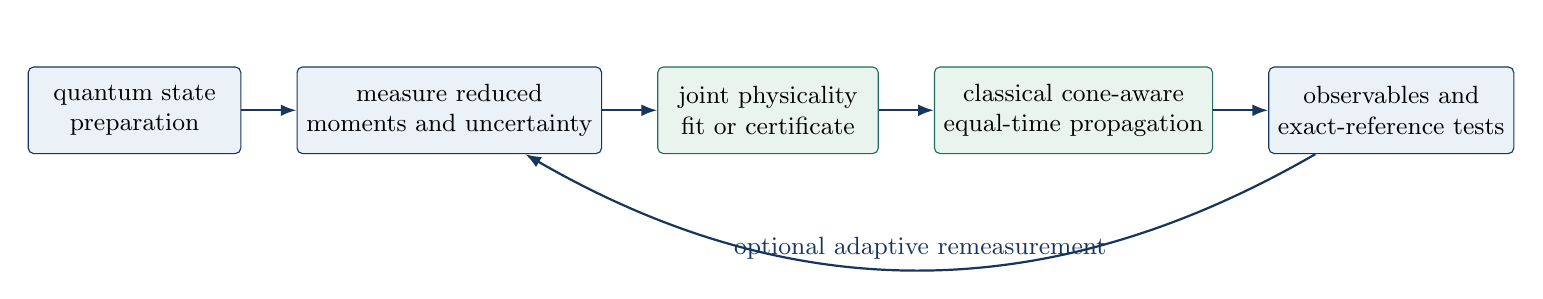
\begin{tikzpicture}[
  node distance=7mm and 7mm,
  every node/.style={font=\small,align=center},
  box/.style={draw=navy,rounded corners=2pt,fill=paleblue,
              minimum width=27mm,minimum height=11mm},
  greenbox/.style={draw=green,rounded corners=2pt,fill=palegreen,
              minimum width=28mm,minimum height=11mm},
  arr/.style={-{Latex[length=2mm]},thick,navy}
]
\node[box] (prep) {quantum state\\preparation};
\node[box,right=of prep] (meas) {measure reduced\\moments and uncertainty};
\node[greenbox,right=of meas] (cert) {joint physicality\\fit or certificate};
\node[greenbox,right=of cert] (prop) {classical cone-aware\\equal-time
propagation};
\node[box,right=of prop] (obs) {observables and\\exact-reference tests};
\draw[arr] (prep)--(meas);
\draw[arr] (meas)--(cert);
\draw[arr] (cert)--(prop);
\draw[arr] (prop)--(obs);
\draw[arr,bend left=30] (obs) to node[above]{optional adaptive remeasurement}
(meas);
\end{tikzpicture}%
}
\caption{Proposed quantum/classical contract.  Quantum estimation does not
remove the need for representability: finite-shot moments should enter the
classical dynamics with an uncertainty-aware physicality certificate.}
\label{fig:quantum}
\end{figure*}

Finite-shot estimates can violate \(\MB\succeq0\) even when the underlying
state is physical.  A measurement-stage fit can solve
\[
\begin{aligned}
\underset{\widehat\rho,\widehat B,\widehat N,\widehat A,\widehat C}
{\text{minimize}}\quad&
\lVert \widehat m-m_{\rm raw}\rVert_{\Sigma^{-1}}^2,\\
\text{subject to}\quad&
0\preceq\widehat\rho\preceq\I,\quad
\Tr\widehat\rho=N_{\rm e},\\
&
\MB(\widehat N,\widehat A)\succeq0,
\end{aligned}
\tag{7.5}
\]
where \(\Sigma\) is the measurement covariance.  This separates noisy initial
moment reconstruction from dynamical cone correction.

\commentarybox{The quantum algorithm and the stability solution are two parts
of one workflow.  The first supplies reduced objects with uncertainty; the
second propagates them inside the domain in which those objects can represent
a physical state.  Neither part substitutes for the other.}

\flowlead{Decision tree for the next result}

\begin{enumerate}
  \item If the direct QP preserves the cones but creates unacceptable energy
  drift, add the energy equality/slack and report feasibility.
  \item If the direct QP passes but the \(C\)-level QP fails, retain the direct
  QP as a reference and diagnose the relative-degree or controllability
  obstruction.
  \item If both keep the cones but disagree strongly with exact observables,
  the second-order closure needs revision rather than a stronger controller.
  \item If both improve exact agreement, expand the parameter sweep and
  cutoff study.
  \item If a bounded physical solution remains sensitive after all
  convergence tests, begin the Lyapunov and bifurcation program.
  \item If quantum moment noise dominates the cone margin, improve measurement
  allocation and the uncertainty-aware fit before interpreting dynamical
  differences.
\end{enumerate}

\flowlead{Acceptance criterion for completion}

The causal diagnosis for the pinned protocol is mostly complete.  The
stability program is complete only after one correction passes:
\[
\boxed{
\begin{gathered}
0\preceq\rho(t)\preceq\I,\quad \MB(t)\succeq0,\\
\text{bounded amplitudes and controlled energy drift},\\
\text{improved exact-dimer agreement},\\
\text{cutoff and solver convergence}
\end{gathered}}
\tag{7.6}
\]
over the declared parameter and time window.

\warningbox{Until Eq.~(7.6) is demonstrated, the cone corrections remain
candidate constructions.  Their derivations are ready for implementation;
their scientific acceptance remains future work.}

\part{Synthesis and research frontier}

\flowlead{Causal chain}

\begin{figure*}[t]
\centering
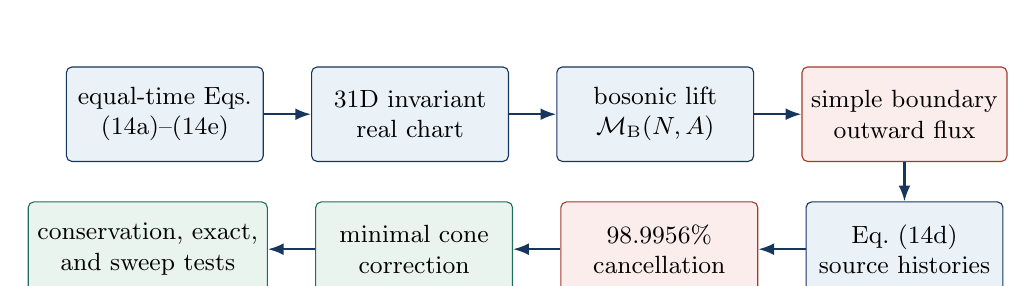
\begin{tikzpicture}[
  node distance=5mm and 6mm,
  every node/.style={font=\small,align=center},
  box/.style={draw=navy,rounded corners=2pt,fill=paleblue,
              minimum width=25mm,minimum height=12mm},
  warn/.style={draw=brick,rounded corners=2pt,fill=palered,
              minimum width=25mm,minimum height=12mm},
  prop/.style={draw=green,rounded corners=2pt,fill=palegreen,
              minimum width=25mm,minimum height=12mm},
  arr/.style={-{Latex[length=2mm]},thick,navy}
]
\node[box] (eqs) {equal-time Eqs.\\(14a)--(14e)};
\node[box,right=of eqs] (scalar) {31D invariant\\real chart};
\node[box,right=of scalar] (mom) {bosonic lift\\\(\MB(N,A)\)};
\node[warn,right=of mom] (cross) {simple boundary\\outward flux};
\node[box,below=of cross] (hist) {Eq.~(14d)\\source histories};
\node[warn,left=of hist] (cancel) {\(98.9956\%\)\\cancellation};
\node[prop,left=of cancel] (qp) {minimal cone\\correction};
\node[prop,left=of qp] (tests) {conservation, exact,\\and sweep tests};

\draw[arr] (eqs)--(scalar);
\draw[arr] (scalar)--(mom);
\draw[arr] (mom)--(cross);
\draw[arr] (cross)--(hist);
\draw[arr] (hist)--(cancel);
\draw[arr] (cancel)--(qp);
\draw[arr] (qp)--(tests);
\end{tikzpicture}
\caption{The argument map.  Each arrow corresponds to a distinct verification:
source transcription, coordinate invariance, moment representability, event
refinement, variation-of-constants reconstruction, correction feasibility,
and physical validation.}
\label{fig:argument}
\end{figure*}

\begin{enumerate}
  \item The source theory evolves five reduced objects rather than the full
  many-body density operator.
  \item The correlation object \(C\) carries memory because its formal
  solution is a propagated source history.
  \item A 13D scalar projection is readable but omits a generated anomalous
  field; the 31D chart closes the tested matrix directions.
  \item Physical bosonic moments must satisfy
  \(\MB(N,A)\succeq0\).
  \item The residual-subtracted exact-contraction trajectory reaches the
  boundary at Eq.~(5.1) with outward derivative Eq.~(5.2).
  \item Equation~(14b) supplies that derivative directly.
  \item Equation~(14d) supplies it historically through \(C\).
  \item The dominant histories are the Eq.~(112) correlation subtraction and
  bare Pauli blocking, which nearly cancel.
  \item The early cone exit is therefore sensitive to a small mismatch
  between large histories.
  \item The state-dependent full-matrix barrier preserves the sampled cone
  through \(t=20\); the energy-neutral chart also retains post-pulse energy
  stability.
\end{enumerate}

\flowlead{Translation table}

\begin{tabularx}{\linewidth}{@{}p{0.25\linewidth}Y@{}}
\toprule
Phrase & Operational meaning \\
\midrule
Object space & The mathematical set declaring the allowed type, symmetry, and
dimension of a variable.\\
Scalarization & A real coordinate chart for matrix objects, together with an
invariance claim that must be tested.\\
Physical cone & The set of moment matrices whose quadratic forms remain
nonnegative.\\
Boundary flux & The derivative of the newly zero eigenvalue along its null
mode.\\
Direct contribution & A term that appears in the current derivative of the
monitored object.\\
Causal history & A source propagated from its creation time through the same
homogeneous correlation dynamics.\\
Residual subtraction & The constant modification
\(F(x,t)\mapsto F(x,t)-F(x_0,0)\).\\
Cone-aware correction & A minimal state-dependent velocity change satisfying
a tangent or barrier constraint.\\
Strange attractor & A bounded invariant attracting set with chaotic structure,
not an unbounded or post-cone-escape trajectory.\\
\bottomrule
\end{tabularx}

\flowlead{What is known, proposed, and open}

\begin{tabularx}{\linewidth}{@{}p{0.20\linewidth}Y@{}}
\toprule
Status & Statement\\
\midrule
Reproduced &
The 31D pinned protocol crosses the bosonic moment cone with the time, flux,
and source histories reported in Part~V.\\
Reproduced &
The paired normal and anomalous Eq.~(14d) histories nearly cancel at that
event; the Eq.~(112)/bare-Pauli pair controls the residual.\\
Reproduced &
The structured energy-neutral moment barrier preserves the sampled fermionic
and bosonic cones through \(t=20\) with post-pulse energy drift
\(2.54\times10^{-6}\).\\
Proposed &
The correlation-level high-order barrier is a well-defined candidate
correction acting on the diagnosed memory channel.\\
Open &
Which correction best preserves representability, boundedness, conservation,
and exact-reference accuracy across a parameter sweep.\\
Open &
Whether a corrected physical trajectory exhibits any positive asymptotic
Lyapunov exponent or strange attractor.\\
Open &
Whether an analytically useful fixed-point stability boundary can be factored
for the full 31D dimer closure.\\
\bottomrule
\end{tabularx}

\flowlead{Reproduction and source provenance}

The primary theory source is the June 2026 arXiv preprint
\emph{Open-quantum-system theory of non-Markovian electron--phonon dynamics}
by Riva, Simoni, and Ping~\cite{riva2026}.  The dimer scalar maps and
Eq.~(112) convention were taken from the local working document
\sourcepath{/Users/jakestrobel/Downloads/Dynamics_on_the_Hubbard_DIMER.pdf}.
The matrix audit and boundary calculation are implemented under
\sourcepath{paper_5/src/paper5/stability/}.  The detailed working-evidence
report is
\sourcepath{output/pdf/paper_v_scalar_stability_diagnostic.pdf}.
The vector plots and event tables were regenerated from the version-7
diagnostic manifest, whose source hashes record the exact working tree.

The main local reproduction command is:
{\footnotesize
\begin{verbatim}
cd paper_5
export PYTHONPATH=src
python3 -m paper5.stability.reproduce \
  --lambda-ep 1.5 --gamma 0.5 --drive 1.0 \
  --time-step 0.01 --final-time 140
\end{verbatim}
}
The stability test suite and report-generation workflow certify the exact
boundary and history tables.

\warningbox{The reproduced evidence retains working-project status.
Paper-facing adoption requires a separate scientific decision.}

\part*{Post-reading mastery quiz}

\textit{Instructions.} Choose one answer, state why it is correct, and name
one tempting alternative.

% Quiz source map:
% P1 Secs 3, P2 Secs 5.2-5.4, P3 Sec 3.5, P4 Sec 7.5,
% P5 Sec 7.6, P6 Secs 3.2-3.4, P7 Sec 4.4, P8 Sec 2.5,
% P9 Secs 2.9/5.3, P10 Part 6, P11 Eq 4.3, P12 Eq 4.7,
% P13 Eq 4.13, P14 Eq 6.3, P15 Eq 5.11.

\flowlead{Conceptual knowledge}

\qhead{P1}{Why is the 31D scalar model preferable for the final cone
diagnostic?}
\choiceblock
{It has fewer variables than the 13D model.}
{It is an explicit real coordinate chart that retains every generated dimer
matrix direction used by the audit.}
{It replaces quantum moments by classical probabilities.}
{It guarantees exact many-body dynamics.}
\confidence

\qhead{P2}{Why is Eq.~(14d) assigned zero \emph{direct} boundary flux but
nonzero causal responsibility?}
\choiceblock
{Equation~(14d) is turned off at the boundary.}
{Its nonlinear terms vanish for every trajectory.}
{It changes only the coherent phonon \(B\).}
{\(\MB\) depends directly on \(N,A\), while Eq.~(14d) first changes \(C\),
whose history then drives Eqs.~(14b)--(14c).}
\confidence

\qhead{P3}{What is the most accurate interpretation of Eq.~(112), written
\(\dot x=F(x,t)-F(x_0,0)\)?}
\choiceblock
{A constant vector-field modification that pins the selected initial
coordinate before the drive.}
{An adaptive reduction of the ODE solver step size.}
{A proof that the initial moments are an exact fixed point of the source
closure.}
{A projection of every step onto the exact many-body state.}
\confidence

\qhead{P4}{Which observation would be required before the phrase ``strange
attractor'' becomes scientifically plausible?}
\choiceblock
{One coordinate exceeds \(10^4\).}
{The instantaneous Jacobian has a positive eigenvalue once.}
{A bounded physical invariant set supports converged chaotic diagnostics.}
{Two initial conditions separate after the bosonic cone has already been
crossed.}
\confidence

\qhead{P5}{What is the proposed role of the quantum stage?}
\choiceblock
{Replace the cone constraints with shot noise.}
{Prepare states and estimate reduced moments, with uncertainty passed to a
classical physicality fit and propagation stage.}
{Integrate the classical 31D ODE without measuring any observables.}
{Guarantee that the second-order closure equals exact dynamics.}
\confidence

\qhead{P6}{What did adding only the relative anomalous coordinate pair
\((m_{\rm R},m_{\rm I})\) establish?}
\choiceblock
{The 13D slice was exactly invariant.}
{The full 31D closure was unnecessary.}
{Bosonic positivity was guaranteed for all time.}
{Equation~(14c) generated an omitted direction, and the 15D projection matched
that minimal matrix sector while remaining incomplete.}
\confidence

\flowlead{Terminology}

\qhead{P7}{What is the ``boundary flux'' at a simple bosonic
cone crossing?}
\choiceblock
{The trace of \(C\)}
{The norm of the complete ODE state}
{\(v^\dagger\dot\MB v=\dot\lambda_{\min}\)}
{\(\det\rho\) at the initial time}
\confidence

\qhead{P8}{Which source is called the bare Pauli-blocking source?}
\choiceblock
{\(-\ii(\I-\rho)G_q^{\mathsf T}\rho\)}
{\(-\ii(\omega_q-\omega_{q'})N_{qq'}\)}
{\(-F(x_0,0)\) in every sector}
{\(-\ii\omega_qB_q\)}
\confidence

\qhead{P9}{What is a variation-of-constants history in the attribution
calculation?}
\choiceblock
{A new trajectory obtained by deleting all other sources.}
{The final value of a source without propagation.}
{A finite-difference perturbation of the initial condition.}
{The contribution generated by one source and transported through the common
time-ordered homogeneous evolution.}
\confidence

\qhead{P10}{What makes a correction ``cone-aware'' here?}
\choiceblock
{It acts whenever any coordinate is nonzero.}
{Its activation and constraint use the physical cone margin and its boundary
velocity.}
{It removes every nonlinear term.}
{It makes the Hamiltonian diagonal.}
\confidence

\flowlead{Mathematical identities}

\qhead{P11}{Which lift jointly tests normal and anomalous bosonic moments?}
\choiceblock
{\(\begin{psmallmatrix}\rho&0\\0&\I-\rho\end{psmallmatrix}\)}
{\(\begin{psmallmatrix}N&A\\A^\dagger&N\end{psmallmatrix}\)}
{\(\begin{psmallmatrix}N^{\mathsf T}&A^\ast\\A&\I+N\end{psmallmatrix}\)}
{\(\begin{psmallmatrix}B^\dagger B&C\\C^\dagger&\rho\end{psmallmatrix}\)}
\confidence

\qhead{P12}{For one mode with normal moment \(n\) and anomalous moment \(m\),
which inequality follows from \(\MB\succeq0\)?}
\choiceblock
{\(|m|^2\leq n(n+1)\)}
{\(|m|\leq n-1\)}
{\(n^2+|m|^2=1\)}
{\(m=0\)}
\confidence

\qhead{P13}{At a simple boundary eigenpair \(\MB v=0\), which identity gives
the first-order cone motion?}
\choiceblock
{\(\dot\lambda_{\min}=\Tr\dot\MB\)}
{\(\dot\lambda_{\min}=v^\dagger\dot\MB v\)}
{\(\dot\lambda_{\min}=\det\dot\MB\)}
{\(\dot\lambda_{\min}=\lVert\dot\MB\rVert_{\Frob}\)}
\confidence

\qhead{P14}{For an unstructured Hermitian velocity correction with unit
null mode \(v\), which minimum-Frobenius-norm solution enforces
\(v^\dagger(D+\Delta D)v\geq\kappa\)?}
\choiceblock
{\(\Delta D=-D\)}
{\(\Delta D=\kappa\I\) in every case}
{\(\Delta D=(v^\dagger Dv-\kappa)vv^\dagger\)}
{\(\Delta D=[\kappa-v^\dagger Dv]_+vv^\dagger\)}
\confidence

\qhead{P15}{Which expression measures the cancellation fraction of signed
history contributions \(f_\alpha\)?}
\choiceblock
{\(\sum_\alpha f_\alpha/\sum_\alpha f_\alpha^2\)}
{\(\max_\alpha|f_\alpha|/\sum_\alpha|f_\alpha|\)}
{\(1-\left|\sum_\alpha f_\alpha\right|/
\sum_\alpha|f_\alpha|\)}
{\(\sum_\alpha|f_\alpha|/\left|\sum_\alpha f_\alpha\right|\)}
\confidence

\clearpage
\part*{Transfer-and-repair work}

These are intentionally unsolved.  They are the bridge from understanding the
diagnosis to producing the next scientific result.

\flowlead{T1: Derive the structured lift adjoint}

Choose an explicit ten-real-coordinate basis for
\((\Delta\dot N,\Delta\dot A)\) at \(Q=2\).  Construct the matrix of
\(\mathcal S\) in Eq.~(6.5), derive its real Frobenius adjoint, and show how
the covector \(a_j=v^\dagger\mathcal S(e_j)v\) is obtained without numerical
differentiation.  State the rank condition under which a simple outward mode
is instantaneously controllable.

\flowlead{T2: Extend the verified direct cone QP}

The pure structured lift, simple-mode minimum-norm solution, full matrix
barrier, and energy-neutral null-space restriction now have regression tests.
Extend the pinned \(t=20\) trajectory through the amplitude-validation
horizon.  Repeat it across solver tolerances, maximum steps, phonon cutoffs,
pulse amplitudes, \(\gamma\), and \(\lambda\); log barrier multipliers,
constraint counts, and activity intervals together with every physicality and
energy metric.

\flowlead{T3: Correlation-level relative degree}

For
\[
h(x)=\lambda_{\min}[\MB(N,A)],
\]
differentiate \(\dot h\) once more along the 31D vector field.  Isolate the
coefficient multiplying the correlation control \(u\), including the
eigenvector-derivative contribution or an equivalent spectral-projector
formula.  Identify states where \(L_gL_fh=0\), because those states cannot be
repaired by an instantaneous Eq.~(14d) control of this form.

\flowlead{T4: Separate amplitude control from cone control}

Run a sector sweep
\[
\alpha_C\in\{0,0.25,0.5,0.75,1\}
\]
in Eq.~(6.17), then compare it with the direct QP and correlation-level QP.
For each case report the first cone event, maximum amplitude, energy drift,
and exact-observable error.  Determine whether any constant \(\alpha_C\)
provides both long-time amplitude stability and early cone preservation.

\flowlead{T5: Fixed-point and local closed-form analysis}

Use the undriven symmetry-reduced 31D equations to solve
\(F(x_\ast,0)=0\) on every connected branch accessible from the exact
contractions.  Compute the exact block Jacobian, factor its characteristic
polynomial where possible, and compare the linear prediction
\(e^{J_\ast t}\delta x(0)\) with nearby numerical trajectories before any cone
event.  Distinguish a saddle, Hopf-type crossing, and nonnormal transient
growth.

\flowlead{T6: Quantum moment certification}

Construct a simulated-shot experiment for the moments in Eq.~(7.3).
Propagate the empirical covariance \(\Sigma\) into a confidence interval for
\(\lambda_{\min}(\MB)\).  Implement the constrained fit in Eq.~(7.5), and
compare raw, naively clipped, and statistically weighted physical estimates.
Report bias, variance, cone-margin coverage, and downstream observable error.

\flowlead{T7: Chaos gate}

Only for a corrected trajectory that passes Eq.~(7.6), calculate a converged
Lyapunov spectrum.  Demonstrate independence from integrator tolerance and
orthonormalization interval, verify boundedness and cone preservation, and
construct an appropriate Poincar\'e section if the drive is periodic.  State
what additional evidence would be required before using the phrase
``strange attractor.''

\flowlead{T8: Closure adequacy test}

If the cone controller remains persistently active, treat that activity as a
model diagnostic.  Compare its correction direction with the moment residual
obtained from exact many-body propagation.  Determine whether a specific
higher-order cumulant predicts the missing inward flux.  This task asks
whether the right remedy is control of the existing closure or enlargement of
the closure.

\clearpage
\section*{References}

\begin{thebibliography}{9}

\bibitem{riva2026}
G.~Riva, J.~Simoni, and Y.~Ping,
\newblock ``Open-quantum-system theory of non-Markovian electron--phonon
dynamics,''
\newblock \emph{arXiv:2606.22233} (2026),
\newblock \url{https://arxiv.org/abs/2606.22233}.

\bibitem{hornjohnson}
R.~A. Horn and C.~R. Johnson,
\newblock \emph{Matrix Analysis}, 2nd ed.,
\newblock Cambridge University Press (2013).

\bibitem{breuer}
H.-P. Breuer and F.~Petruccione,
\newblock \emph{The Theory of Open Quantum Systems},
\newblock Oxford University Press (2002).

\end{thebibliography}

\pedbox{Companion numerical record.}{Detailed numerical tables, solver
checks, source hashes, and the test manifest are stored in
\sourcepath{output/pdf/paper_v_scalar_stability_diagnostic.pdf} and its
source.}

\clearpage
\appendix
\part*{Detachable solutions}

\flowlead{Answer grids}

\begin{center}
\scriptsize
\setlength{\tabcolsep}{2.2pt}
\begin{tabular}{@{}lccccccccccccccc@{}}
\toprule
&1&2&3&4&5&6&7&8&9&10&11&12&13&14&15\\
\midrule
Entrance&B&D&A&C&B&D&A&C&B&D&C&A&D&B&C\\
Mastery&B&D&A&C&B&D&C&A&D&B&C&A&B&D&C\\
\bottomrule
\end{tabular}
\end{center}

\flowlead{Entrance exam solutions}

\qhead{E1 --- B}{Outside the PSD cone}

The negative eigenvalue is decisive: a Hermitian matrix is positive
semidefinite exactly when \emph{all} eigenvalues are nonnegative.  The
controlling invariant is the quadratic-form condition
\(z^\dagger Xz\geq0\) for every \(z\); choosing the eigenvector of
\(-0.01\) produces a negative value.  The nearest distractor is C, ``on the
boundary,'' because the number is small and close to zero.  A boundary
eigenvalue must equal zero, whereas any strictly negative value, independent
of its size, lies outside the cone.

\qhead{E2 --- D}{The eigenvalue \(\lambda\)}

From \(Xv=\lambda v\) and the normalization \(v^\dagger v=1\),
left-multiplication gives
\(v^\dagger Xv=\lambda v^\dagger v=\lambda\).  The controlling invariant is
the normalized eigenpair identity, which interprets an eigenvalue as the
quadratic form along its eigenmode.  The nearest distractor is B,
\(\lambda^2\), because norms often square amplitudes.  No norm is being taken
here; the expression contains one application of \(X\), so it returns the
eigenvalue itself.

\qhead{E3 --- A}{Electronic expectations are preserved}

The defining property of the partial trace is
\[
\Tr_{\rm e}(\varrho_{\rm e}O_{\rm e})
=\Tr[\varrho(O_{\rm e}\otimes\I_{\rm ph})]
\]
for every electronic observable.
That expectation-value identity is the controlling invariant.  The nearest
distractor is D, ``correlations vanish,'' because the reduced state no longer
displays phonon labels.  The operation removes explicit access to the phonon
factor; it does not assert that the full state was uncorrelated.  Correlations
can affect the reduced electronic state even though they cannot be recovered
from it alone.

\qhead{E4 --- C}{A constrained real coordinate chart}

A Hermitian \(2\times2\) matrix has two real diagonal entries and one complex
off-diagonal entry, hence four real degrees of freedom.  Storing those four
numbers is an exact coordinate representation of the same object.  The
controlling invariant is Hermiticity, which fixes the lower off-diagonal entry
as the conjugate of the upper.  The nearest distractor is A, ``approximated by
a scalar,'' because the implementation uses scalar entries.  A list of
scalars can encode a matrix exactly; approximation begins only if dynamically
generated matrix directions are omitted.

\qhead{E5 --- B}{Separately propagated source histories}

For a linear inhomogeneous equation, variation of constants writes the
solution as the homogeneous propagation of the initial value plus one
integral for each source.  The controlling invariant is superposition:
histories propagated through the same \(U(t,s)\) add exactly to the complete
solution.  The nearest distractor is A, the final eigenvalues of \(L\), because
those eigenvalues can describe local homogeneous growth but cannot determine
when, where, or with what sign each time-dependent source entered the final
state.

\qhead{E6 --- D}{On the PSD cone boundary}

The cone interior is characterized by a strictly positive smallest
eigenvalue, while its boundary contains positive-semidefinite matrices with at
least one zero eigenvalue.  The controlling invariant is
\(\lambda_{\min}(X)=0\) together with continuity from positive values.  The
nearest distractor is A, the cone origin, because the origin is indeed a
boundary point.  It is only one boundary point: a matrix may have one zero
eigenvalue and several positive eigenvalues, so it need not vanish.

\qhead{E7 --- A}{Hermitian}

``Hermitian'' is defined by equality with the adjoint,
\(X=X^\dagger\).  This is the controlling identity and implies a real
spectrum.  The nearest distractor is B, ``unitary,'' because both terms
involve the adjoint.  A unitary matrix instead satisfies
\(X^\dagger X=\I\); it need not equal its adjoint, and its eigenvalues need
not be real.  The two properties can coexist for special matrices, yet their
definitions are distinct.

\qhead{E8 --- C}{Positive semidefinite}

Positive semidefiniteness is exactly the property
\(z^\dagger Xz\geq0\) for every direction \(z\).  That universal quadratic
form is the controlling invariant.  The nearest distractor is B, ``normal,''
because Hermitian matrices are normal and normal matrices have a useful
spectral decomposition.  Normality only requires
\(X^\dagger X=XX^\dagger\); it places no sign restriction on the spectrum or
quadratic form.

\qhead{E9 --- B}{An eigenmode}

The nonzero vector \(v\) satisfying \(Xv=\lambda v\) is an eigenvector, called
an eigenmode here to emphasize the physical direction selected by the
matrix.  The controlling identity is the eigenvalue equation itself.  The
nearest distractor is A, ``a source term,'' because later calculations
project source velocities along \(v\).  The source is the matrix or vector
being projected; \(v\) is the direction used to interrogate it.

\qhead{E10 --- D}{Partial trace}

The partial trace removes one tensor factor while preserving expectation
values for observables on the retained factor.  That expectation-value
property is the controlling invariant.  The nearest distractor is A,
``transpose,'' because both operations visibly rearrange or remove indices
in coordinate expressions.  A transpose only swaps matrix indices within the
same space; it neither removes a Hilbert-space factor nor defines a reduced
state.

\qhead{E11 --- C}{Reverse the order under the adjoint}

The product rule is
\((AB)^\dagger=B^\dagger A^\dagger\).  The reversal is required because
\(\langle x,AB y\rangle=\langle B^\dagger A^\dagger x,y\rangle\).  This inner
product relation is the controlling invariant.  The nearest distractor is A,
which preserves the original order.  It looks plausible if conjugate
transpose is treated entrywise, but the transpose part reverses matrix
multiplication.

\qhead{E12 --- A}{Nonnegative quadratic form in every direction}

For a Hermitian matrix, \(X\succeq0\) is equivalent to
\(z^\dagger Xz\geq0\) for all \(z\), and also to nonnegative eigenvalues.  The
universal quadratic-form condition is the controlling invariant.  The nearest
distractor is D, \(\det X=1\), because determinants summarize eigenvalue
products and are often used in positivity checks for small matrices.  A
positive determinant can arise from two negative eigenvalues and does not
enforce positive semidefiniteness.

\qhead{E13 --- D}{Hermitian, PSD, unit trace}

A density operator must be Hermitian so expectations are real, positive
semidefinite so probabilities are nonnegative, and normalized so total
probability is one.  Those three conditions form the controlling invariant
set.  The nearest distractor is B because a pure-state density operator does
satisfy an additional idempotence condition, but \(\varrho^2=\I\) is not that
condition and would be far too restrictive.  Mixed states are valid density
operators without being projectors.

\qhead{E14 --- B}{Conjugate off-diagonal entries}

Hermiticity requires real diagonal entries and
\(X_{21}=X_{12}^\ast\).  Choice B satisfies exactly that coordinate identity.
The controlling invariant is \(X=X^\dagger\).  The nearest distractor is A,
which would be correct only when \(b\) happened to be real.  Because the
question permits arbitrary complex \(b\), repeating \(b\) without
conjugation makes the matrix complex symmetric rather than necessarily
Hermitian.

\qhead{E15 --- C}{The chain rule}

Along \(\dot x=F(x,t)\), the directional derivative of \(h\) is
\(\dot h=\nabla h(x)\cdot\dot x=\nabla h(x)\cdot F(x,t)\).  The chain rule is
the controlling invariant.  The nearest distractor is A, \(hF\), because a
linear scalar equation can have a product of state and rate.  For a general
diagnostic \(h(x)\), its sensitivity to each coordinate is encoded by the
gradient, which cannot be omitted.

\clearpage
\flowlead{Post-reading mastery solutions}

\qhead{P1 --- B}{The 31D chart retains the generated dimer directions}

The final cone diagnostic needs an invariant coordinate chart: applying the
matrix vector field to an embedded state must not generate omitted directions.
The controlling invariant is the 31D split
\(\R^3\oplus\R^4\oplus\R^4\oplus\R^6\oplus\R^{14}\), whose projection was
checked against every generated matrix direction in the implemented sector.
The nearest distractor is D, ``exact many-body dynamics,'' because a complete
coordinate chart can exactly represent the \emph{chosen closure} while the
closure itself still omits higher moments of the many-body hierarchy.

\qhead{P2 --- D}{Direct dependence and historical dependence are different}

The monitored matrix \(\MB(N,A)\) depends directly only on \(N\) and \(A\),
so its first derivative contains Eqs.~(14b)--(14c) but no explicit
Eq.~(14d) term.  The controlling map chain is
\(C\xrightarrow{14b,14c}(N,A)\xrightarrow{\LB}\MB\): Eq.~(14d) creates the
correlation field that later enters the direct flux.  The nearest distractor
is B, that the nonlinear terms vanish.  Their separate propagated histories
are nonzero; some happen to cancel at the reported boundary.

\qhead{P3 --- A}{A constant vector-field intervention}

Equation~(112) subtracts the fixed vector \(F(x_0,0)\) at every time and
state, making the selected initial velocity zero before the drive.  The
controlling identity is
\(F_{\rm reg}(x,t)=F(x,t)-F(x_0,0)\), which alters the dynamics globally.
The nearest distractor is C, a proof that the initial moments are a source-EOM
fixed point.  The opposite is true: the subtraction is introduced precisely
because the exact contractions generally have a nonzero residual in the
truncated closure.

\qhead{P4 --- C}{A bounded physical invariant set with converged chaos tests}

A strange attractor must be invariant, attracting, bounded, and dynamically
chaotic.  The controlling evidence contract therefore begins with cone
preservation and boundedness, then requires converged Lyapunov and structural
diagnostics.  The nearest distractor is B, a positive instantaneous Jacobian
eigenvalue, because that observation can indicate local amplification.
Instantaneous eigenvalues do not accumulate the tangent dynamics along a
trajectory and can be positive during nonchaotic transient growth.

\qhead{P5 --- B}{Quantum estimation feeds a certified classical stage}

The proposed quantum contract is to prepare a relevant state and estimate the
reduced moments and their uncertainty.  The controlling workflow is
measurement \(\to\) physicality fit or certificate \(\to\) cone-aware
classical propagation.  The nearest distractor is C because a hybrid
algorithm does use a classical ODE, but it cannot integrate that ODE without
the measured state variables.  The quantum stage supplies physical inputs;
it does not replace the classical stability contract.

\qhead{P6 --- D}{The 15D model closes the first omitted anomalous direction}

Equation~(14c) generates a complex relative anomalous mode even when the 13D
embedding sets \(A=0\).  Adding its two real coordinates restores parity for
that minimal sector and proves that the original slice was not invariant.
The controlling equations are Eq.~(3.7).  The nearest distractor is B, that
31D became unnecessary, because other normal, anomalous, coherent, and
correlation directions remain outside the 15D symmetry-reduced chart and are
needed for the full dimer audit.

\qhead{P7 --- C}{The null-mode eigenvalue derivative}

At a simple boundary eigenpair \(\MB v=0\), the boundary flux is
\(v^\dagger\dot\MB v=\dot\lambda_{\min}\).  The controlling invariant is the
first-order eigenvalue perturbation formula, whose sign distinguishes inward
and outward motion.  The nearest distractor is B, the full state norm, because
large amplitudes are an important later diagnostic.  A norm does not identify
which physical fluctuation mode has reached zero or whether its velocity
points outside the PSD cone.

\qhead{P8 --- A}{The occupation--availability source}

The bare Pauli-blocking source is
\(-\ii(\I-\rho)G_q^{\mathsf T}\rho\).  The controlling structure is the
product of an occupied electronic factor \(\rho\), an available factor
\(\I-\rho\), and the coupling, without multiplication by \(N\) or \(A\).
The nearest distractor is C, the Eq.~(112) subtraction, because that history
nearly opposes the bare source in the final flux.  Their numerical opposition
does not make their mathematical origins the same.

\qhead{P9 --- D}{One source propagated through the common homogeneous flow}

A source history is
\(C_\alpha(t)=\int_{t_0}^tU(t,s)S_\alpha(s)\,\dd s\), using the same
time-ordered \(U\) as every other contribution along the realized trajectory.
Superposition is the controlling invariant: the histories and propagated
initial value reconstruct \(C(t)\).  The nearest distractor is A, a rerun with
other sources deleted.  Such an ablation changes \(\rho,N,A,B\) and hence
\(\mathcal L(t)\); it is a counterfactual trajectory, not an exact attribution
of the realized one.

\qhead{P10 --- B}{Use the cone margin and its velocity}

A cone-aware correction monitors
\(h=\lambda_{\min}(\MB)\) and constrains either
\(\dot h=v^\dagger\dot\MB v\) or a higher-order barrier involving \(h\) and
its derivatives.  That state-dependent viability condition is the
controlling invariant.  The nearest distractor is A, activation whenever a
coordinate is nonzero, because physical trajectories generally contain
nonzero moments.  Persistent indiscriminate activation would modify the
source physics even deep in the cone interior.

\qhead{P11 --- C}{The bosonic second-moment lift}

The correct lift is
\(\MB=\begin{psmallmatrix}N^{\mathsf T}&A^\ast\\A&\I+N\end{psmallmatrix}\).
It follows directly from
\(\xi=(\delta b^\dagger,\delta b)^{\mathsf T}\) and
\(\MB=\langle\xi\xi^\dagger\rangle\); the commutator supplies the identity
block.  The nearest distractor is B because it places \(N\) and \(A\) into a
plausible Hermitian block arrangement.  It omits the transpose, conjugation,
and bosonic \(+\I\) required by the operator ordering.

\qhead{P12 --- A}{The one-mode uncertainty inequality}

For
\(\MB=\begin{psmallmatrix}n&m^\ast\\m&n+1\end{psmallmatrix}\), PSD requires
nonnegative principal minors, giving
\(\det\MB=n(n+1)-|m|^2\geq0\).  That determinant condition, together with
\(n\geq0\), is the controlling invariant.  The nearest distractor is D,
\(m=0\), because setting anomalous correlations to zero certainly satisfies
the pair part of the inequality.  It is sufficient in that restricted case,
not necessary for a physical squeezed or correlated state.

\qhead{P13 --- B}{First-order eigenvalue perturbation}

Differentiating \(\MB v=\lambda v\), left-multiplying by \(v^\dagger\), and
using normalization cancels the eigenvector-derivative terms and yields
\(\dot\lambda=v^\dagger\dot\MB v\).  This perturbation identity is the
controlling invariant for a simple eigenvalue.  The nearest distractor is A,
the trace derivative, because the trace is the sum of all eigenvalue
derivatives.  It cannot isolate the newly null mode and can remain positive
while that one eigenvalue moves outward.

\qhead{P14 --- D}{Rank-one positive-part projection}

The constraint deficit is
\(\kappa-v^\dagger Dv\).  If it is positive, the minimum-Frobenius-norm
Hermitian correction points along the unit constraint normal \(vv^\dagger\);
if it is nonpositive, the zero correction is feasible and optimal.  These KKT
conditions give
\(\Delta D=[\kappa-v^\dagger Dv]_+vv^\dagger\).  The nearest distractor is C,
which has the sign reversed and would push an outward velocity farther
outward precisely when repair is needed.

\qhead{P15 --- C}{One minus signed magnitude over absolute magnitude}

The total available magnitude is
\(\sum_\alpha|f_\alpha|\), while the magnitude surviving cancellation is
\(|\sum_\alpha f_\alpha|\).  Their ratio is the uncancelled fraction, so one
minus that ratio is the cancellation fraction.  This decomposition is the
controlling identity.  The nearest distractor is D, which inverts the ratio
and produces a large amplification factor rather than a number between zero
and one measuring cancellation.

\flowlead{Governing relations}

The complete causal account links:
\begin{enumerate}
  \item the ambient spaces of \(\rho,B,N,A,C\);
  \item the non-Markovian memory carried by Eq.~(14d);
  \item the readable, non-invariant 13D projection and the invariant 31D
  closure;
  \item the physical cone condition \(\MB\succeq0\);
  \item the simple-boundary scalar \(v^\dagger\dot\MB v\);
  \item the direct Eq.~(14b) doorway and the Eq.~(14d) causal history;
  \item the sensitivity induced by the \(98.9956\%\) cancellation;
  \item the direct and correlation-level cone corrections;
  \item the acceptance tests governing scientific adoption;
  \item the quantum estimation stage in the propagation workflow.
\end{enumerate}

\pedbox{Final perspective.}{The important conceptual move is to stop treating
``divergence'' as one phenomenon.  The object spaces reveal the physical
domain; the cone eigenmode locates the first escape; scalar coordinates expose
the term balance; variation of constants identifies the source history; and a
constrained correction turns that diagnosis into a falsifiable next
calculation.}

\end{document}
